\chapter{任意角的三角函数}

\section{弧和角的概念及其度量}

\subsection{任意大小的角}
在平面几何里,每一个角可以看作是由一条射线绕着它
的端点旋转而形成的。射线的端点叫做角的顶点,射线旋转的
开始位置叫做角的始边,终止位置叫做角的终边。如图6.1所
示的角$\alpha$是射线$OA$绕着端点$O$,按着箭头所示的方向旋转
到$OB$所形成。$O$点是角$\alpha$的顶点,射线$OA$和$OB$分别是
角$\alpha$的始边和终边。
\begin{figure}[htp]
    \centering
\begin{tikzpicture}[>=latex]
    \draw (0,0)node[left]{$O$}--(3,0)node[right]{$A$};
    \draw (0,0)--(50:3) node [right]{$B$};
\draw[->, thick] (1,0) arc (0:50:1);
\node at (25:1.25){$\alpha$};
\end{tikzpicture}
    \caption{}
\end{figure}

\begin{figure}[htp]
    \centering
    
        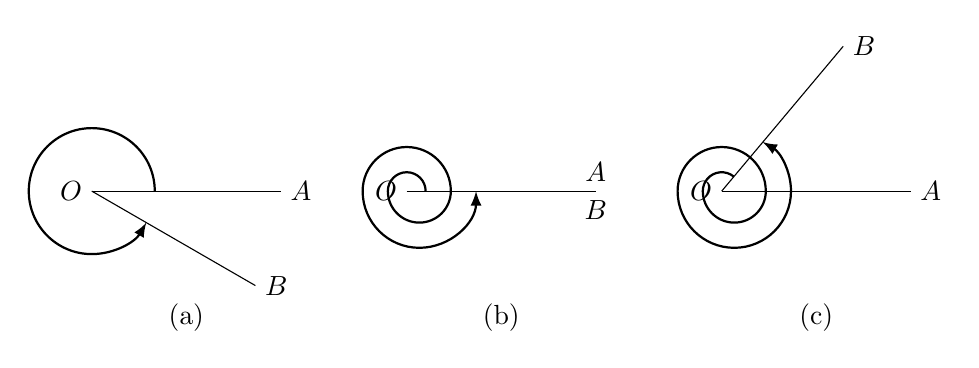
\begin{tikzpicture}[>=latex, scale=.8]
            \begin{scope}
            \draw (0,0)node[left]{$O$}--(3,0)node[right]{$A$};
            \draw (0,0)--(-30:3) node [right]{$B$};
        \draw[->, thick] (1,0) arc (0:360-30:1);
        \node at (1.5,-2){(a)};
    \end{scope}
    \begin{scope}[xshift=5cm]
            \draw (0,0)node[left]{$O$}--(3,0)node[above]{$A$};
          \node at   (3,0)[below]{$B$};
        \draw[thick] (.3,0) arc (0:180:.3);
        \draw[thick] (-.3,0) arc (180:360:.5);
        \draw[thick] (.7,0) arc (0:180:.7);
        \draw[thick,->] (-.7,0) arc (180:360:.9);

        \node at (1.5,-2){(b)};
    \end{scope}
    \begin{scope}[xshift=10cm]
        \draw (0,0)node[left]{$O$}--(3,0)node[right]{$A$};
        \draw (0,0)--(50:3) node [right]{$B$};
        \draw[thick] (50:.3) arc (50:180:.3);
        \draw[thick] (-.3,0) arc (180:360:.5);
        \draw[thick] (.7,0) arc (0:180:.7);
        \draw[thick,->] (-.7,0) arc (180:360+60:.9);
    \node at (1.5,-2){(c)};
\end{scope}
        \end{tikzpicture}
    \caption{}
\end{figure}

射线旋转所形成的角可以是任意大小的角,这也就是
说,一条射线旋转所成的角可以是锐角,钝角,平角,也可
以大于一个平角(图6.2a),也可以绕端点若干周后和开始
的位置重合(图6.2b),也可以旋转若干周又一周的部分
(图6.2c)。

我们还看到射线有两种相反的旋转方向:逆时针方向和
顺时针方向。为了加以区别,我们把按逆时针方向旋转所形
成的角叫做正角,按顺时针方向旋转所形成的角叫做负角。
例如图6.3中以$OA$为始边的角$\alpha=210^{\circ}$, $\beta=-150^{\circ}$, $\gamma=-660^{\circ}$.
\begin{figure}[htp]
    \centering
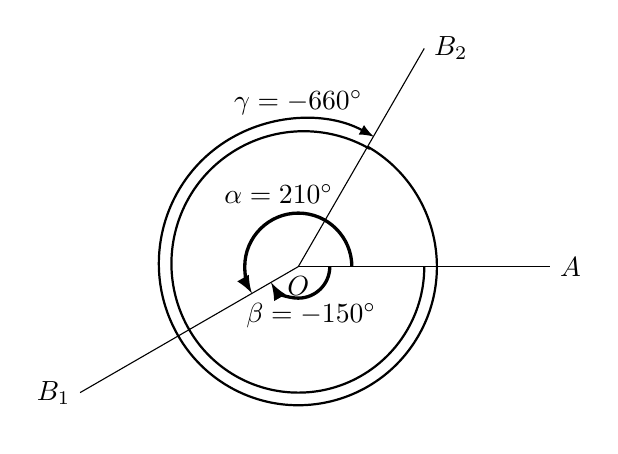
\begin{tikzpicture}[>=latex, scale=.8]
\draw (0,0)node[below]{$O$}--(4,0)node[right]{$A$};
\draw (0,0)--(-150:4)node[left]{$B_1$};    
\draw (0,0)--(60:4)node[right]{$B_2$};    
\draw[->, very thick] (.5,0) arc (0:-150:.5);
\node at (-75:.8){$\beta=-150^{\circ}$};

\draw[->, very thick] (.85,0) arc (0:210:.85);
\node at (105:1.2){$\alpha=210^{\circ}$};

\draw[thick] (2,0) arc (0:-150:2) ;
\draw[thick] (-150:2) arc (-150:-150-150:2.1) ;
\draw[thick] (60:2.2) arc (60:-150:2.2);
\draw[->, thick] (-150:2.2) arc (-150:-150-149:2.3);
\node at (0,2.6){$\gamma=-660^{\circ}$};


\end{tikzpicture}
    \caption{}
\end{figure}

如果射线$OA$没有
作任何旋转,仍留在开
始的位置,那么我们也
把它看成一个角,叫做\textbf{零角}。

这样,我们把角的概念推广到了任意的
角,包括正角、负角和零角。

我们这样引进来的广义角的概念,是由下列三个因素组
成:“始边”、“旋转方向”、“旋转量”。旋转量的大小
通常是以度数或弧度数来表示。

和角的概念对应的是弧的概念。

我们已经讨论了任意大小的角,现在再来讨论任意大小
的弧。

圆弧可以看做是射线上的一点(不与端点重合),随着
射线旋转所形成的轨迹。

\begin{figure}[htp]
    \centering
\begin{tikzpicture}
\draw (4,0)node[right]{$A$}--(0,0)node[left]{$O$}--(40:4)node[above]{$B$};
\draw (1.5,0)node[below]{$M$} arc (0:40:1.5) node[above]{$M'$};
\end{tikzpicture}
    \caption{}
\end{figure}




如图6.4所示,弧$\wideparen{MM'}$是射线$OA$上的$M$点,随着射
线$OA$旋转,由起始位置到$OB$时所形成的轨迹。显然,对
于任意角$\alpha$的终边的每个位置,都有$M$点划出的弧$\wideparen{MM'}$
和它对应。和规定角的正负一样,我们规定:当射线上的一
点按逆时针方向旋转时,该点所划出的弧为正的;按顺时针
方向旋转时,该点所划出的弧为负的,这样规定就使正、负
角和正、负弧对应起来。

再来规定角和它所对应弧的量数。在平面几何里,我们曾规定把圆
周分成360等分,每一份叫做一度的弧,一度弧所对的圆心角叫做一度的
角。因此,一个圆弧含有多少度、分、
秒,它所对圆心角也含有多少度、
分、秒,即弧与其所对应的圆心角有完全相同的量数。例如
圆心角是$500^{\circ}$的角时,它所对的弧就是$500^{\circ}$的弧;圆心角是$-300^{\circ}$时,它所对的弧也是$-300^{\circ}$.

\subsection{角的度量}
角的度量是取一个确定的角作为度量单位,利用它来量
所有的角。用周角的$\frac{1}{360}$
作为度量单位的叫做“度”。在高
等数学和其它基础科学理论系统中也常用弧度作为度量圆弧
和角的单位。

在弧度制中,取等于半径长的圆弧作为单位弧长。这样
的弧叫做一弧度弧。用一弧度弧度量同一个圆上的圆弧所得
到的量数叫做这个圆弧的弧度数,这也就是说给定圆弧的弧
度数等于圆弧的弧长和半径的比值:
\begin{equation}
    \alpha=\frac{\ell}{R}
\end{equation}
这里$\alpha$是圆弧的弧度数,$\ell$是弧长,$R$是圆的半径。

我们指出圆心角所张的圆弧的弧度数由这个角的大小决
定,而和圆的半径长短无关。

事实上,从几何里知道,在
圆心角相同时,两个圆上的弧长
的比等于它们的半径长的比(图6.5), 即
\[\frac{\wideparen{A_1B_1}}{\wideparen{A_2B_2}}=\frac{R_1}{R_2}\]
或\[\frac{\wideparen{A_1B_1}}{R_1}=\frac{\wideparen{A_2B_2}}{R_2}\]
这就是说,两个圆弧$\wideparen{A_1B_1}$, $\wideparen{A_2B_2}$的弧度数是相同的。

\begin{figure}[htp]
    \centering
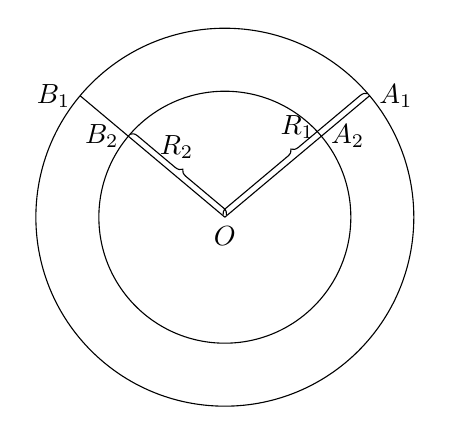
\begin{tikzpicture}[scale=.8]
\draw (0,0) circle (2);
\draw (0,0) circle (3);
\draw (0,0)--(40:3);
\draw (0,0)--(140:3);

\node at (40:2)[right]{$A_2$};
\node at (40:3)[right]{$A_1$};
\node at (140:2)[left]{$B_2$};
\node at (140:3)[left]{$B_1$};
\node at (0,0)[below]{$O$};

\draw[decorate,decoration={brace,raise=1pt}] (0,0)--node[above=3pt]{$R_1$}(40:3);
\draw[decorate,decoration={brace,raise=1pt}] (140:2)--node[above=3pt]{$R_2$}(0,0);
\end{tikzpicture}
    \caption{}
\end{figure}

因此,一个圆心角所对的弧的弧度数可以表示这个角的
大小,我们也把圆心角所对的圆弧的弧度数称为这个角的弧
度数。

\begin{blk}{定义}
    以一个角为圆心角,这个角所对的弧的长和这个
弧的半径长之比,叫做这个角的弧度数。
\end{blk}

当弧长等于半径时,这个比值等于1, 因此,在弧度制
里,度量一个角时,我们规定:

长度等于半径的圆弧所对的圆心角叫做1弧度角。换言
之,一弧度圆弧所对的圆心角叫做1弧度角。

这样,由(6.1)推得
\begin{equation}
    \ell=aR
\end{equation}
即圆弧长等于这圆弧的弧度数(或这弧所对圆心角的弧度数)
和半径长的乘积。特别地,单位圆上的弧长等于它的弧度数。

利用(6.1)还可以接计算一些特殊角的弧度数。

当弧长等于圆周长$C=2\pi R$时,这个比值等于$2\pi$, 因
此,
\[\begin{split}
    \text{周角}&=  \frac{2\pi R}{R}=2\pi \text{弧度}\\
    \text{平角}&=\frac{1}{2} \text{周角}=\pi \text{弧度}\\
    \text{直角}&=\frac{1}{4}\text{周角}=\frac{\pi}{2}\text{弧度}\\
    45^{\circ}&=\frac{1}{2}\text{直角}=\frac{\pi}{4}\text{弧度}\\
    30^{\circ}&=\frac{1}{3}\text{直角}=\frac{\pi}{6}\text{弧度}\\
    60^{\circ}&=\frac{1}{3}\text{平角}=\frac{\pi}{8}\text{弧度}\\
\end{split}\]

\begin{rmk}
角的量数是以弧度数表示的,通常只写出数值不
写出单位,以后我们都将单位“弧度”二字省略不写。例如
平角$=\pi$弧度就写成平角$=\pi$。但是千万不要误解平角就是
圆周率$3.1415926\cdots$。
\end{rmk}

度与弧度的互化。

因为平角$=180^{\circ}=\pi$, 所以$1^{\circ}=\frac{\pi}{180}
\approx 0.017453$。$A^{\circ}$的角相应的弧度数:
\[\begin{split}
    \alpha&=\frac{A\pi}{180}\\
    1'&=\left(\frac{1}{60}\right)^{\circ}=\frac{1}{60}\left(\frac{\pi}{180}\right)\approx 0.00029088\\
    1\text{(弧度)}&=\frac{180^{\circ}}{\pi}=57.295^{\circ}\approx 3438'\approx 206265''
    = 57^{\circ}17'45''
\end{split}\]
$\alpha$弧度的角相应的度数:
\[A^{\circ}=\frac{a\cdot 180^{\circ}}{\pi}\]

下表给出一些常见角的弧度和它们的近似值:
\begin{center}
\begin{tabular}{cccccccc}
\hline
度 & $30^{\circ}$ & $45^{\circ}$ & $60^{\circ}$ & $90^{\circ}$ & $180^{\circ}$ & $270^{\circ}$ & $360^{\circ}$\\
\hline
弧度 & $\frac{\pi}{6}$   & $\frac{\pi}{4}$   & $\frac{\pi}{3}$   & $\frac{\pi}{2}$   & $\pi$   & $\frac{3}{2}\pi$  & $2\pi$\\
近似值 & 0.5236   & 0.7854   & 1.0472   & 1.5708   & 3.1416   & 4.7124   & 6.2832\\
\hline
\end{tabular}
\end{center}

\begin{example}
    化$67^{\circ}30'$为弧度。
\end{example}

\begin{solution}
\[67^{\circ}30'=67.5^{\circ}=\frac{\pi}{180}\x 67.5=\frac{3}{8}\pi \; \text{(弧度)}\]
\end{solution}

\begin{example}
    化$\frac{3}{5}\pi$弧度为度。
\end{example}

\begin{solution}
  \[\frac{3}{5}\pi= \frac{180^{\circ}}{\pi}\x\frac{3}{5}\pi=108^{\circ}  \]  
\end{solution}

\begin{example}
    两皮带轮的半径$R_1=20$, $R_2=30$, 求它们的转速
    之比(图6.6)。
\begin{figure}[htp]
    \centering
    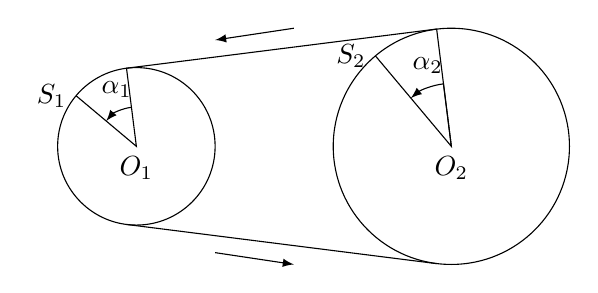
\begin{tikzpicture}[>=latex]
\draw (0,0) circle (1);
\draw (4,0) circle (1.5);
\node at  (0,0) [below]{$O_1$};
\node at  (4,0) [below]{$O_2$};
\draw (140:1)node[left]{$S_1$}--(0,0)--(97.2:1)--+(7.2:3.97)--(4,0)--+(130:1.5)node[left]{$S_2$};
\draw (-97.2:1)--+(-7.2:3.97);
\draw[->] (97.2:.5) arc (97.2:140:.5);
\draw[->] (4,0)--+(97.2:.8) arc (97.2:130:.8);
\node at (-.25,.5)[above]{$\alpha_1$};
\node at (4-.3,.8)[above]{$\alpha_2$};

\draw[<-]  (1,1.35)--(2,1.5);
\draw [->] (1,-1.35)--(2,-1.5);

    \end{tikzpicture}
    \caption{}
\end{figure}
\end{example}

\begin{solution}
    因为在相同的时间内,两轮周上转过的弧长相等,
    即$S_1=S_2$, 在弧度制下:
\[S_1=\alpha_1 R_1,\qquad S_2=\alpha_2 R_2\]
$\therefore\quad \alpha_1R_1=\alpha_2R_2 \quad \Rightarrow\quad \frac{\alpha_1}{\alpha_2}=\frac{R_2}{R_1}=\frac{30}{20}$

$\therefore\quad \alpha_1:\alpha_2=3:2 $
\end{solution}

\begin{example}
    地球的半径为6400公里,在同一经线上,甲、乙两
地的距离为150公里,试求甲、乙两地纬度差。
\end{example}


\begin{solution}
设$\theta$为甲、乙两地纬度差,则
\[\begin{split}
    \theta &= \frac{150}{6400}\approx 0.0234\\
    &=0.0234\x\frac{180^{\circ}}{\pi}\\
    &\approx 0.0234\x 3438'\\
    &\approx 13^{\circ}14'
\end{split}\]

答: 两地纬度差为$13^{\circ}14'$。
\end{solution}

\begin{ex}
\begin{enumerate}
    \item 把下列各角的度数化为弧度数:
\begin{multicols}{3}
    \begin{enumerate}
    \item $2^{\circ}$
    \item $5^{\circ}$
    \item $7^{\circ}30'$
    \item $12^{\circ}30'$
    \item $22.5^{\circ}$
    \item $200^{\circ}$
    \item $320^{\circ}$
    \item $14^{\circ}24'$
    \item $86^{\circ}45'$
    \item  $157^{\circ}30'$
\end{enumerate}
\end{multicols}

\item 把下列各角的弧度数化为度数:
 \begin{multicols}{3}
    \begin{enumerate}
        \item $0.4800$
        \item $0.0099$ 
        \item $2.6400$
        \item $\frac{3}{5}\pi$
        \item $\frac{4}{5}\pi$
        \item $\frac{\pi}{15}$
        \item $\frac{\pi}{10}$
        \item $3\pi$
\end{enumerate}
\end{multicols}

\item 已知$200^{\circ}$的圆心角所对的弧长等于50cm, 求圆的
半径。
\item 轮子每秒旋转$\frac{5}{18}$
弧度,20秒钟内转了多大角度?
\item 一个大钟的长针长2尺8寸.20秒间针端走了几寸?
\item 扇形弧长为20cm, 半径为15cm, 求扇形面积。
\item 地球半径为6400公里,地面上一弧所对球心角为$1'$,
问弧长若干公里?
\end{enumerate}
\end{ex}

\subsection{始边和终边相同的角}
今后我们常在直角坐标系里讨论角,并把角放在下面的
标准位置:使角的顶点与坐标原点重合,角的始边与$x$轴的
正半轴重合,角的终边在第几象限,就把这个角叫做第几象
限角(或说这个角属于第几象限)。如图6.7(1)中,
$\frac{\pi}{6}$, $\frac{13\pi}{6}$
和$-\frac{11\pi}{6}$
都是第一象限的角。在图6.7(2)中,
$-\frac{\pi}{3}$, $\frac{5\pi}{3}$
都是第四象限的角。

\begin{figure}[htp]
    \centering
\begin{tikzpicture}[>=latex]
\begin{scope}
    \draw[->](-2,0)--(2,0)node[right]{$x$};
    \draw[->](0,-2)--(0,2)node[right]{$y$};
\draw (0,0)--(30:2.5)node[right]{$B$};
\draw[->] (.75,0) arc (0:30:.75);
\draw[->] (1,0) arc (0:-330:1);
\node at (.2,-.2){$O$};
\node at (15:1){$\tfrac{\pi}{6}$};
\node at (2,.5){$\tfrac{13\pi}{6}$};
\node at (.5,1.2){$-\tfrac{11\pi}{6}$};
\draw(1.5,0) arc (0:270:1.5);
\draw [->] (0,-1.5) arc (270:384:1.7);
\node at (0,-2.5){(1)};
\end{scope}
\begin{scope}[xshift=6cm]
    \draw[->](-2,0)--(2,0)node[right]{$x$};
    \draw[->](0,-2)--(0,2)node[right]{$y$};
    \draw (0,0)--(-60:2.5)node[right]{$B$};
    \draw[->] (.75,0) arc (0:-60:.75);
    \draw[->] (1,0) arc (0:300:1);
    \node at (.2,.2){$O$};
    \node at (-30:1){$-\tfrac{\pi}{3}$};
    
\node at (1,1){$\tfrac{5\pi}{3}$};
\node at (0,-2.5){(2)};

\end{scope}
\end{tikzpicture}   
    \caption{}
\end{figure}


在图6.7(1)中可以看到$\frac{13\pi}{6}$与$-\frac{11\pi}{6}$都和$\frac{\pi}{6}$的角终边相同。
$\frac{13\pi}{6}$和$-\frac{11\pi}{6}$
可以写成下列形式:
\[2\pi+\frac{\pi}{6},\qquad -2\pi+\frac{\pi}{6}\]
显然,除了这两个角以外,与
的角终边相同的角还有:
\[\begin{split}
    2\x 2\pi+\frac{\pi}{6},&\qquad -2\x 2\pi+\frac{\pi}{6}\\
    3\x 2\pi+\frac{\pi}{6},&\qquad -3\x 2\pi+\frac{\pi}{6}\\
\cdots\cdots\qquad &\qquad\qquad \cdots\cdots
\end{split}\]
所有和$\frac{\pi}{6}$
的角终边相同的角,连同$\frac{\pi}{6}$
在内,可以用下式表示:
\[2k\pi+\frac{\pi}{6},\quad (k\in\mathbb{Z})\]
当$k=1$时,它表示$\frac{\pi}{6}$的角;$k=1$时,它表示$\frac{13\pi}{6}$的角;$k=-1$时,它表示$-\frac{11\pi}{6}$的角。

一般地,所有和$\alpha$角终边相同的角,连同$\alpha$在内,可
以用式子$2k\pi+\alpha\; (k\in\mathbb{Z})$来表示。

由此可见,具有相同始边和终边的角不止一个,而是无
穷多个,它们之间彼此相差整数周(正的或负的)即$2\pi$的整数
倍。实际上,相同始边和终边的角是由无穷多个角组成的集
合。与$\alpha$终边相同的角($\alpha$角处在标准位置)的集合可记作:
\[\{\beta|\beta=2k\pi+\alpha,\; k\in\mathbb{Z}\}\quad  \text{(若$\alpha$以弧度制给出)}\]
或
\[\{\beta|\beta=k\cdot 360^{\circ}+\alpha,\; k\in\mathbb{Z}\}\quad  \text{(若$\alpha$以度数制给出)}\]


\begin{example}
    在$0^{\circ}$到$360^{\circ}$的范围内,找出与下列各角终边相同
的角,并判定下列各角是哪个象限的角。
\[-120^{\circ},\qquad 640^{\circ},\qquad -950^{\circ}12'\]

\end{example}


\begin{solution}
\begin{enumerate}
    \item $\because\quad -120^{\circ}=-360^{\circ}+240^{\circ}$
    
$\therefore\quad -120^{\circ}$的角与$240^{\circ}$的角的终边相同,它是第
三象限的角。
\item $\because\quad 640^{\circ}=360^{\circ}+280^{\circ}$

$\therefore\quad 640^{\circ}$的角与$280^{\circ}$的角的终边相同,它是第四象限
的角。

\item $\because\quad -950^{\circ}12'=-3x360^{\circ}+129^{\circ}48'$

$\therefore\quad -950^{\circ}12'$的角与$129^{\circ}48'$的角的终边相同,它是
第二象限的角。
\end{enumerate}
\end{solution}

\begin{example}
写出与下列各角终边相同的角的集合$S$, 并把$S$
中$-2\pi$到$4\pi$间的角写出来:
\[\frac{\pi}{3},\qquad -\frac{\pi}{4},\qquad \frac{15\pi}{7}\]
\end{example}

\begin{solution}
\begin{enumerate}
    \item 
$S=\left\{\beta \Big|\beta =2k\pi+\frac{\pi}{3},\; k\in\mathbb{Z}\right\}$

$S$中在$-2\pi$到$4\pi$间的角:
\begin{itemize}
    \item 当$k=-1$时,$\beta =-2\pi+\frac{\pi}{3}=\frac{-5\pi}{8}$
    \item 当$k=0$时,$\beta=\frac{\pi}{3}$ 
    \item 当$k=1$时,$\beta =2\pi+\frac{\pi}{3}=\frac{7\pi}{3}$
\end{itemize}

\item $S=\left\{\beta \Big|\beta =2k\pi-\frac{\pi}{4},\;k\in\mathbb{Z}\right\}$

$S$中在$-2\pi$到$4\pi$间的角:
\begin{itemize}
    \item 当$k=0$时,$\beta =-\frac{\pi}{4}$
    \item 当$k=1$时,$\beta =2\pi-\frac{\pi}{4}=\frac{7\pi}{4}$
    \item 当$k=2$时,$\beta =4\pi-\frac{\pi}{4}=\frac{15\pi}{4}$
\end{itemize}

\item $S=\left\{\beta \Big|\beta =2k\pi+\frac{15\pi}{7},\; k\in\mathbb{Z}\right\}$

$S$中在$-2\pi$到$4\pi$间的角:
\begin{itemize}
    \item 当$k=-2$时,$\beta =-4\pi+\frac{15\pi}{7}=-\frac{13\pi}{7}$
    \item 当$k=-1$时,$\beta =-2\pi+\frac{15\pi}{7}=\frac{\pi}{7}$
    \item 当$k=0$时,$\beta=\frac{15\pi}{7}$
\end{itemize}
\end{enumerate}    
\end{solution}

如果处在标准位置的角的终边落在坐标轴上,那么如何
写出终边相同的角呢?下面我们来研究这个问题。

\begin{enumerate}
    \item 终边落在$x$轴的正向上,这些角的量数为
\[2n\pi\quad  (n\in\mathbb{Z})\]
\item 终边落在x轴的负向上,这些角的量数
\[2n\pi +\pi =(2n+1)\pi\quad  (n\in\mathbb{Z})\]
把1、2结合起来,量数为$k\pi\;  (k\in\mathbb{Z})$的角的终边
落在$x$轴上,在$k$为偶数时,终边落在$x$轴的正向上;在$k$
为奇数时,终边落在$x$轴的负向上。
\item 终边落在$y$轴的正向上,这些角的量数为
\[2n\pi +\frac{\pi}{2}\quad (n\in\mathbb{Z})\]
\item 终边落在$y$轴的负向上,这些角的量数为
\[-\frac{\pi}{2}+2nx=(2n-1)\pi +\frac{\pi}{2}\quad (n\in\mathbb{Z})\]
把3、4结合起来,量数为$k\pi +\frac{\pi}{2}\; (k\in\mathbb{Z})$的
角的终边落在$y$轴上,在$k$为偶数时,终边落在$y$轴的正向
上,在$k$为奇数时,终边落在$y$轴的负向上。
\end{enumerate}

量数为$k\cdot \frac{\pi}{2}\; (k\in\mathbb{Z})$的角的终边,或落在$x$轴上,或落在$y$轴上。在$k=0,1,2,3,4,5,\ldots$时,终边依次落
在$z$轴正向、$y$轴正向、$x$轴负向、$y$轴负向、$x$轴正向、$y$
轴正向……在$k=-1,-2,-3,-4,-5,\ldots$
时,终边依次落在$y$轴负向、$x$轴负向、$y$轴正向、$x$轴正
向、$y$轴负向……

此外,若$\alpha$的终边落在右半平面(一、四象限),则满足
\[-\frac{\pi}{2}+2k\pi<\alpha<\frac{\pi}{2}+2k\pi\quad (k\in\mathbb{Z})\]
若$\alpha$的终边落在上半平面(一、二象限),则满足
\[2k\pi <\alpha<(2k+1)\pi \]

以上这些表示法希望大家熟悉,因为以后经常要用到。

\begin{ex}
\begin{enumerate}
    \item 在度数制下,写出下面处在标准位置的终边相同的
    角。
        \begin{enumerate}    \begin{multicols}{2}
    \item $30^{\circ}$
    \item 终边落在$x$轴正向上;
    \item 终边落在$x$轴负向上;
    \item 终边落在$x$轴上;
    \item 终边落在$y$轴正向上;
    \item 终边落在$y$轴负向上;
    \item 终边落在$y$轴上;    \end{multicols}
    \item 角$\alpha$的终边落在左半平面上;
    \item 角$\alpha$的终边落在下半平面上。     
    \end{enumerate}

    
    \item 把下列角放在标准位置上,用量角器作出下列各角,
    并指出它们是哪个象限的角。
    \[-55^{\circ},\qquad -265^{\circ},\qquad 400^{\circ} ,\qquad 1000^{\circ},\qquad -512^{\circ} \]

    \item 当时钟上指出3点,6点和8点的时候,写出分针
    与时针所成角的一般形式。
    \item 试求出下列处在标准位置的各角的最小正同边角及
    最大负同边角,并说明各角为何象限角:
    \[1140^{\circ},\qquad 1680^{\circ},\qquad -1290^{\circ},\qquad -1510^{\circ}\]
\item 写出与下列各角终边相同的角的集合,并把集合中
在$-4\pi$ 到$2\pi$ 间的角写出来:
\[\frac{\pi}{4},\qquad -\frac{\pi}{6},\qquad \frac{36\pi}{5},\qquad -\frac{8\pi}{7}\]
\end{enumerate} 
\end{ex}

\subsection{单位圆}
\begin{blk}{定义}
    以坐标原点为圆心,半径长为1的圆叫做单位圆。
它上面任一弧的长度恰好等于弧度数。
\end{blk}
 
如图6.8, 单位圆交坐标轴于四个点$A(1,0)$、$B(0,1)$、
$A_1(-1,0)$、$B_1(0,-1)$。过$A$作单位圆的切线$\ell$, 在$\ell$上这
样来建立坐标系:取$A$为原点,取向上的方向为正向,单
位等于半径长,这样$\ell$就是一条实数轴。我们已经知道实数
轴上的点和全体实数是一一对应的。

\begin{figure}[htp]
    \centering
\includegraphics[scale=.6]{fig/6-8.PNG}
    \caption{}
\end{figure}



现在把数轴$\ell$设想为一
条无限长而没有伸缩性的丝
线,把数轴$\ell$正的那一半按
反时针方向来包卷单位圆,
而用这条数轴负的那一半按
顺时针方向包卷于单位圆上。设$S_1$是数轴$\ell$正的那一半上的一点(图6.8),当
$\ell$包卷到圆上后,此点就落到
单位圆上的$P_1$点,此时$S_1$
点的坐标是单位圆上弧$\wideparen{AP_1}$
的长或$\wideparen{AP_1}$的弧度数,也是
$\wideparen{AP_1}$所对圆心角$\theta$的弧度数。如
果数轴$\ell$上的一点坐标是负的,那么它就是$\ell$的负半轴按顺
时针方向包卷在单位圆上的负弧或它所对负圆心角的弧度
数,通过数轴在单位圆上的包卷,我们建立了数轴上一切点的
坐标和处在标准位置的圆心角$\theta$的弧度数之间的一一对应,
并且由于它们的基本单位相等,于是$\theta$角的弧度数就可以从
包卷在单位圆上的数轴$\ell$上的点的坐标直接读出来。

我们必须注意,在数轴$\ell$上,坐标相差$2\pi$ 的或相差$2\pi$ 
整数倍的那些点,当把$\ell$包卷在单位圆上时,都位于同一
点,例如$P_1$点是弧长$S_1$达到的一点,那么弧长等于$S_1\pm 2\pi,
S_1\pm 4\pi ,\ldots$的弧,当$\ell$包卷在单位圆上时也达到同一个
点$P_1$, 这就说明了数轴上的点和单位圆上的点是多一对应。
于是数轴$\ell$上的任意两个实数$S_1,S_2$和单位圆上同一个点
对应的充要条件是:
\[S_1-S_2=2n\pi \qquad  (n\in\mathbb{Z})\]
我们把上述两种对应复合在一起得到:
\begin{align*}
    \text{实数}\mathbb{R}& \longleftrightarrow  \{\theta|\text{标准位置有向角的弧度数}\}  \tag{一一对应}\\
& \longrightarrow \{(x,y)|x^2+y^2=1\} \tag{多一对应}
\end{align*}

这里$(x,y)$是单位圆上点的坐标。
我们在下面将应用这种对应关系来研究三角函数的许多
性质。并且把角的三角函数与实变数的三角函数统一起来。


\begin{example}
    在单位圆上作出对应于下列各数的点:
\[0,\quad \frac{\pi}{6},\quad \frac{\pi}{3},\quad \frac{\pi}{2},\quad \frac{2\pi}{3},\quad \frac{5\pi}{6},\quad \pi,\quad \frac{7\pi}{6},\quad \frac{4\pi}{3},\quad \frac{3\pi}{2},\quad \frac{5\pi}{3},\quad \frac{11\pi}{6},\quad 2\pi\]
\end{example}

\begin{solution}
    这些数中每相邻两数的差是$\frac{\pi}{6}$,
即在单位圆上以
相邻两数为端点的弧都相等,因此我们将单位圆12等分后,就
得到对应于上列各数的点(图6.9)。
\begin{figure}[htp]
    \centering
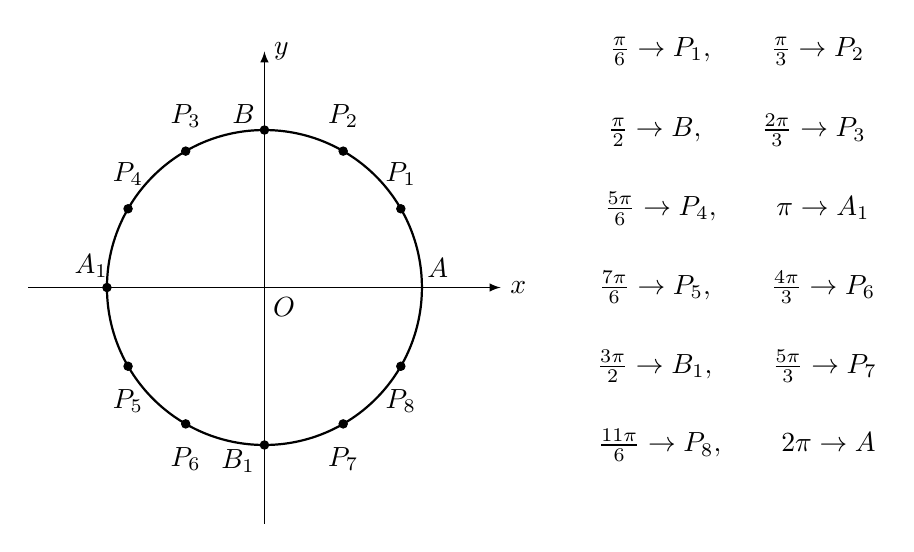
\begin{tikzpicture}[>=latex]
    \draw[->] (-3,0)--(3,0)node[right]{$x$};
    \draw[->] (0,-3)--(0,3)node[right]{$y$};
\draw[thick] (0,0) circle(2);

    \draw (1*30:2) [fill=black] circle (1.5pt) node[above=5pt]{$P_1$};
    \draw (2*30:2) [fill=black] circle (1.5pt) node[above=5pt]{$P_2$};
    \draw (3*30:2) [fill=black] circle (1.5pt);
    \draw (4*30:2) [fill=black] circle (1.5pt) node[above=5pt]{$P_3$};
    \draw (5*30:2) [fill=black] circle (1.5pt) node[above=5pt]{$P_4$};
    \draw (6*30:2) [fill=black] circle (1.5pt);
    \draw (7*30:2) [fill=black] circle (1.5pt) node[below=5pt]{$P_5$};
    \draw (8*30:2) [fill=black] circle (1.5pt) node[below=5pt]{$P_6$};
    \draw (9*30:2) [fill=black] circle (1.5pt);
    \draw (10*30:2) [fill=black] circle (1.5pt) node[below=5pt]{$P_7$};
    \draw (11*30:2) [fill=black] circle (1.5pt) node[below=5pt]{$P_8$};
   
\node at (2.2,0)[above]{$A$};   
\node at (-2.2,0)[above]{$A_1$};
\node at (0,2.2)[left]{$B$};   
\node at (0,-2.2)[left]{$B_1$};
\node at (0.25,-.25){$O$};  

\node at (6,3){$\frac{\pi}{6}\to P_1,\qquad \frac{\pi}{3}\to P_2$};
\node at (6,2){$ \frac{\pi}{2}\to B,\qquad \frac{2\pi}{3}\to P_3$};
\node at (6,1){$\frac{5\pi}{6}\to P_4,\qquad \pi\to A_1$};
\node at (6,0){$\frac{7\pi}{6}\to P_5,\qquad \frac{4\pi}{3}\to P_6$};
\node at (6,-1){$\frac{3\pi}{2}\to B_1,\qquad \frac{5\pi}{3}\to P_7$};
\node at (6,-2){$\frac{11\pi}{6}\to P_8,\qquad 2\pi\to A$};

\end{tikzpicture}
    \caption{}
\end{figure}
\end{solution}

\begin{example}
在数轴$\ell$上找到和单位圆上$(0,1)$点对应的一切实
数。
\end{example}

\begin{solution}
在单位圆上$B$点的坐标是$(0,1)$, $\wideparen{AB}$的弧长是$\frac{\pi}{2}$,
因此在数轴$\ell$上和$(0,1)$点对应的一切实数是:$\frac{\pi}{2}+2k\pi\; (k\in\mathbb{Z})$。

\end{solution}

\begin{ex}
\begin{enumerate}
   \item 在单位圆上找出与实数0, $\frac{\pi}{2}$, $-\frac{\pi}{2}$,$\pi$对应的点$P_1$、$P_2$、$P_3$、$P_4$. 并写出与$\angle AOP_1$、$\angle AOP_2$、$\angle AOP_3$、
$\angle AOP_4$对应的一切实数的一般形式。


\item \begin{enumerate}
\item 在单位圆上找出分别与下面各实数0、$\frac{\pi}{6}$、$\frac{\pi}{4}$、$\frac{\pi}{3}$、$\frac{\pi}{2}$对应的点$P_0$、$P_1$、$P_2$、$P_3$、$P_4$。
\item 分别写出$P_0$、$P_1$、$P_2$、$P_3$、$P_4$各点的直角坐标。
\item 与下面各实数对应的点,哪些和$P_0$、$P_1$、$P_2$、$P_3$、$P_4$关于坐标轴对称?哪些关于原点对称?并写出它们的直
角坐标。
\end{enumerate} 
\end{enumerate}
\[\frac{2\pi}{3},\quad \frac{3\pi}{4},\quad \frac{5\pi}{6},\quad \pi,\quad \frac{7\pi}{6},\quad \frac{5\pi}{4},\quad \frac{4\pi}{3},\quad \frac{3\pi}{2},\quad \frac{5\pi}{3},\quad -\frac{\pi}{4},\quad \frac{11\pi}{6}\]
\end{ex}

\section{任意角的三角函数}
在描述和研究有关转动和振动的实际问题的时候,我们
就要研究任意角的三角函数,下面我们来研究任意角的三角
函数。

\subsection{任意角三角函数的定义}
如图6.10, 在角$\alpha$的终边上任意取一点$P$(不是坐标
系的原点)。

以坐标系的原点为起点,$P$为终点的有向线段$\Vec{OP}$叫做
$P$点的向量半径或旋转半径。

设$P$点的坐标是$(x,y)$, 它和原点的距离为$r>0$(即
旋转半径$\Vec{OP}$的长),横坐标$x$与纵坐标$y$的正负是由
$P$点所在的象限来确定的。距离$r$总是正的,并且
\[r=\sqrt{x^2+y^2}\]

\begin{figure}[htp]
    \centering
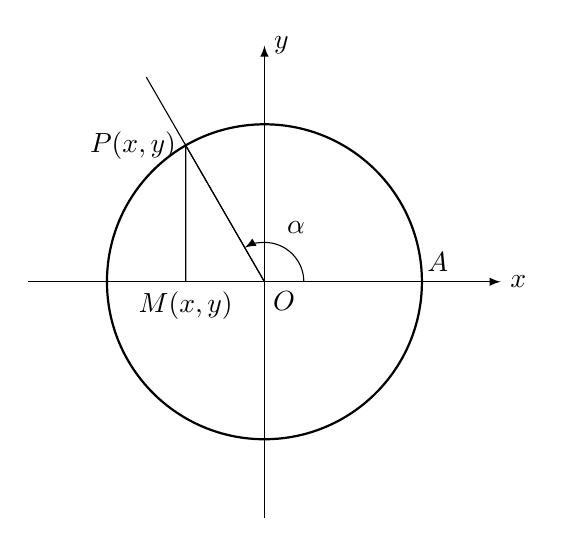
\begin{tikzpicture}[>=latex]
    \draw[->] (-3,0)--(3,0)node[right]{$x$};
    \draw[->] (0,-3)--(0,3)node[right]{$y$};
\draw[thick] (0,0) circle(2);
\draw (0,0)--(120:3);
\draw (0,0)--(120:2)node[left]{$P(x,y)$}--(-1,0)node[below]{$M(x,y)$};
   
\node at (2.2,0)[above]{$A$};   
\node at (.25,-.25){$O$};
\draw[->] (.5,0) arc (0:120:.5);
\node at (60:.8){$\alpha$};
\end{tikzpicture}
    \caption{}
\end{figure}

\begin{blk}{定义}
    \begin{enumerate}
\item $\frac{y}{r}$叫做角$\alpha$的正弦,记作$\sin\alpha$, 即
$\sin\alpha=\frac{y}{r}$;
\item $\frac{x}{r}$叫做角$\alpha$的余弦,记作$\cos\alpha$, 即$\cos\alpha=\frac{x}{r}$;
\item $\frac{y}{x}$
叫做角$\alpha$的正切,记作$\tan\alpha$, 即$\tan\alpha=\frac{y}{x}$;
\item $\frac{x}{y}$叫做角$\alpha$的余切,记作$\cot\alpha$, 即$\cot\alpha=\frac{x}{y}$;
\item $\frac{r}{x}$
叫做角$\alpha$的正割,记作$\sec\alpha$, 即$\sec\alpha=\frac{r}{x}$;
\item $\frac{r}{y}$
叫做角$\alpha$的余割,记作$\csc\alpha$, 即$\csc\alpha=\frac{r}{y}$。        
    \end{enumerate}
\end{blk}

对于确定的角$\alpha$,$\frac{y}{r},\; \frac{x}{r},\; \frac{y}{x},\; \frac{x}{y},\; \frac{r}{x},\; \frac{r}{y}$
这六个比值的大小,和我们在$\alpha$角的终边上所取$P$点的位置没有关系,如图6.11中,$P_1(x_1,y_1)$点为角$\alpha$终边上
另一点,$P_1$到原点$O$的距离为$r_1$,$x$和$x_1$、$y$和$y_1$的符号
相同,因为$\triangle POM\sim \triangle P_1OM_1$,所以
\[\begin{split}
   & \frac{y_1}{r_1}=\frac{y}{r},\qquad \frac{x_1}{r_1}=\frac{x}{r},\qquad \frac{y_1}{x_1}=\frac{y}{x}\\
   &\frac{x_1}{y_1}=\frac{x}{y},\qquad  \frac{r_1}{x_1}= \frac{r}{x},\qquad \frac{r_1}{y_1}=\frac{r}{y}
\end{split}\]

\begin{figure}[htp]
    \centering
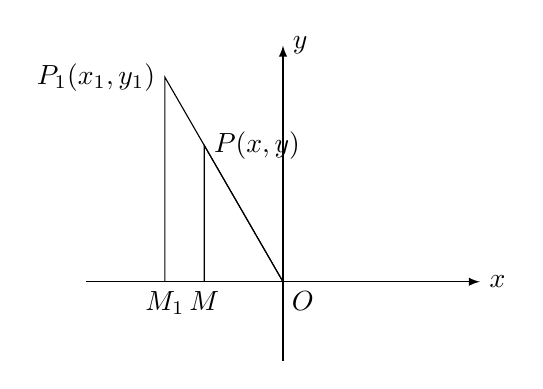
\begin{tikzpicture}[>=latex]
    \draw[->] (-2.5,0)--(2.5,0)node[right]{$x$};
    \draw[->] (0,-1)--(0,3)node[right]{$y$};
\draw (0,0)--(120:3)node[left]{$P_1(x_1,y_1)$}--(-1.5,0)node [below]{$M_1$};
\draw (0,0)--(120:2)node[right]{$P(x,y)$}--(-1,0)node [below]{$M$};
\node at (.25,-.25){$O$};
\end{tikzpicture}
    \caption{}
\end{figure}

这就是说,对于确定的角 $\alpha$, $\sin\alpha$、$\cos \alpha$、$\tan \alpha$、$\cot \alpha$、
$\sec\alpha$、$\csc\alpha$
都有确定的值,因为它们的值是随着 $\alpha$变化而
变化的,当 $\alpha$角取确定值的时候,它们的值也相应地唯一确
定,所以,角 $\alpha$的正弦、余弦、正切、余切、正割和余割都
是角 $\alpha$的函数,这些函数都叫做三角函数。

很明显,当角 $\alpha$是锐角或钝角时,上面三角函数的定义
和锐角、钝角三角函数的定义完全一样,所以锐角、钝角三
角函数定义是任意角三角函数定义的特例。

根据任意角三角函数定义,可以看出
\[\sec\alpha=\frac{1}{\cos\alpha},\qquad \csc \alpha=\frac{1}{\sin\alpha},\qquad \cot \alpha=\frac{1}{\tan\alpha}\]

今后我们主要研究
$\sin \alpha$、 $\cos \alpha$、$\tan \alpha$、$\cot \alpha$ 四个函数。

\begin{example}
    已知单位圆中旋转半径$OP$和$OX$轴正方向成
$300^{\circ}$角,求 $\sin300^{\circ}$, $\cos300^{\circ}$, $\tan 300^{\circ}$, $\cot300^{\circ}$。

\end{example}

\begin{solution}
    设$OP$的端点$P$的坐标是$(x,y)$. 作直线$PM\bot OX$轴于$M$点,$A$点是单位圆与$OX$轴的交点$(1,0)$, 联结
$P,A$(图6.12). 在$\triangle OPA$中,

$\because\quad OP=OA=1,\quad \angle POA=360^{\circ}-300^{\circ}=60^{\circ}$

$\therefore\quad \triangle OPA$是等边三角形,因此,$PM$垂直平分$OA$,
$|x|=|OM|=\frac{1}{2}$
\[\begin{split}
    |y|&=|PM|=\sqrt{|OP|^2-|OM|^2}\\
&=\sqrt{1-\left(\frac{1}{2}\right)^2}=\frac{\sqrt{3}}{2}
\end{split}\]

\begin{figure}[htp]
    \centering
\begin{tikzpicture}[>=latex]
    \draw[->] (-3,0)--(3,0)node[right]{$x$};
    \draw[->] (0,-3)--(0,3)node[right]{$y$};
\draw[thick] (0,0) circle(2);
\draw (0,0)--(-60:2)--(2,0);
\draw (1,0)node[above]{$M(\tfrac{1}{2},0)$}--(-60:2)node[below]{$P(x,y)$};
   
\node at (2.5,0)[below]{$A(1,0)$};   
\node at (-.25,-.25){$O$};
\draw[->] (.5,0) arc (0:300:.5);
\node at (150:.8){$300^{\circ}$};
\end{tikzpicture}
    \caption{}
\end{figure}

又$\because\quad P$点在第四象限,$\therefore\quad P$点坐标是
\[x=\frac{1}{2},\qquad y=-\frac{\sqrt{3}}{2}\]
由此求得
\[\sin300^{\circ}=-\frac{\sqrt{3}}{2},\qquad 
\cos300^{\circ}=\frac{1}{2}\]
\[
\tan300^{\circ}=-\sqrt{3},\qquad 
\cot300^{\circ}=-\frac{1}{\sqrt{3}}=-\frac{\sqrt{3}}{3}\]
\end{solution}


\begin{example}
    $$\cos 0=1,\qquad \sin 0=0,\qquad \cos\frac{\pi}{2}=0,\qquad \sin\frac{\pi}{2}=1$$
    \[\cos\pi=-1,\qquad \sin\pi=0,\qquad \cos\frac{3\pi}{2}=0,\qquad \sin\frac{3\pi}{2}=-1\]
\end{example}

\subsection{数值变数的三角函数与三角函数的定义域}
在数学中两个变数之间的函数可以表示不同物理量或几
何量之间的函数关系,例如,数学中的二次函数$y=ax^2$,
如果$a=1$, $a$表示正方形的边长的数值,$y$就表示正方形的
面积数值;但是当
$a=\frac{1}{2}g$
时,$x$表示自由落体下降的时
间,则$y$表示下降的距离。同样,有许多物理或技术问题,
常常要用到的三角函数,其中的自变量就不一定是角或弧而
是时间或长度等,所以为了满足科学技术上的需要,就必需
把角的三角函数扩充为变数$x$的三角函数。

假设$x$是在函数定义域内的任意实数,根据前节
讨论知,对应此实数有一个量数是$x$的角或弧(用弧度作
单位),而对应于该角又有它的各三角函数值,由于这种关
系,对于任意实数$x$就有完全确定的三角函数值$y$与之对
应,于是得到了一个数值变数的三角函数。

\begin{blk}{定义}
 变数$x$的三角函数就是具有弧度数$x$的角(或
弧)的三角函数。    
\end{blk}


\begin{example}
    若$x=1.54$, 求$\sin x$的值。
\end{example}

\begin{solution}
    因为$\sin1.54=\sin1.54\text{弧度}$,
又 $1.54\text{弧度}\approx 88^{\circ}14'$,

所以
$\sin1.54\approx \sin88^{\circ}14'\approx 0.9995$
\end{solution}

在任意大小的角、弧及数之间所能建立的对应,使得我
们可以认为三角函数是角的函数,或是弧的函数,或是数的
函数,其中变数由我们处理,可以解释为角或解释为弧,或
解释为数。

现在给每个三角函数确定它的定义域:

设数值$\alpha$, 有单位圆上的点$P$与之对应(如图6.13),
那么$P$点的坐标是
\[x=\cos\alpha,\qquad y=\sin\alpha\]

\begin{figure}[htp]
    \centering
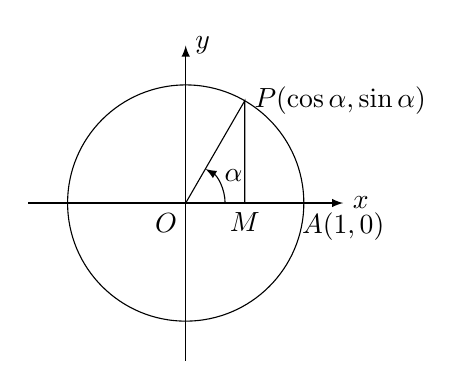
\begin{tikzpicture}[>=latex]
\draw[->] (-2,0)--(2,0)node[right]{$x$};
\draw[->] (0,-2)--(0,2)node[right]{$y$};
\draw (0,0) circle (1.5);
\draw (0,0)--(60:1.5)node[right]{$P(\cos\alpha,\sin\alpha)$}--(1.5/2,0)node[below]{$M$};
\node at (-.25,-.25){$O$};\node at (2,0)[below]{$A(1,0)$};
\draw[->] (.5,0) arc (0:60:.5);
\node at (30:.7){$\alpha$};
\end{tikzpicture}
    \caption{}
\end{figure}


因此:
\[\tan\alpha=\frac{y}{x}=\frac{\sin\alpha}{\cos\alpha},\qquad \cot\alpha=\frac{x}{y}=\frac{\cos\alpha}{\sin\alpha}\]
\[ \sec\alpha=\frac{1}{x}=\frac{1}{\cos\alpha},\qquad \csc\alpha=\frac{1}{y}=\frac{1}{\sin\alpha}\]

\begin{enumerate}
    \item 函数 $\cos\alpha$和$\sin\alpha$的定义域是开区间$-\infty<\alpha<+\infty$,
    即$(-\infty,+\infty)$, 这是因为 $\cos\alpha$和$\sin\alpha$是单位圆上对应
    于数$\alpha$的点$P$的横坐标和纵坐标,它们对于任何实数$\alpha$都
    有明确的值。
\item 函数$\tan\alpha$的定义域是除去形如$\frac{\pi}{2}+k\pi\; (k\in\mathbb{Z})$的数的实数集:
    \[\left\{\alpha\Big|\alpha\in\mathbb{R},\; \alpha\ne \frac{\pi}{2}+k\pi, \; k\in\mathbb{Z} \right\} \]
    即正切的定义域是无限个开区间组成的一个集:
\[\cdots, \left(-\frac{3\pi}{2},-\frac{\pi}{2}\right), \left(-\frac{\pi}{2},\frac{\pi}{2}\right), \left(\frac{\pi}{2},\frac{3\pi}{2}\right),\left(\frac{3\pi}{2},\frac{5\pi}{2}\right),\cdots\]
这是因为$\tan\alpha =\frac{y}{x}$
是单位圆上$P$点
的纵坐标对横坐标之比,唯有当$x=0$时它失去意义,单位圆
上与$x=0$对应的点只有$(0,1)$和$(0,-1)$, 与$(0,1)$点对应的
一切实数是$\alpha=\frac{\pi}{2}+2k\pi\; (k\in\mathbb{Z})$, 与$(0,-1)$点对应的一
切实数是$\alpha=-\frac{\pi}{2}+2k\pi\; (k\in\mathbb{Z})$, 和$(0,1)$点、$(0,-1)$
点这两点对应的一切实数可以合并写成:
\[\alpha=\frac{\pi}{2}+k\pi\qquad  (k\in\mathbb{Z})\]
\item 函数$\cot\alpha$的定义域是除去形如$k\pi\;  (k\in\mathbb{Z})$的数的实
数集:$\{\alpha|\alpha\in\mathbb{R},\; \alpha\ne k\pi ,k\in\mathbb{Z}\}$, 即余切的定义域是无
限个开区间组成的一个集:
\[\cdots, (-\pi ,0),(0,\pi ),(\pi ,2\pi ),\cdots\]
\item 函数$\sec\alpha$的定义域与正切函数$\tan\alpha$的定义域$\left\{\alpha\Big|\alpha\in\mathbb{R},\;  \alpha\ne \frac{\pi}{2}+k\pi ,k\in\mathbb{Z}\right\}$相同。
\item 函数$\csc\alpha$的定义域与余切函数$\cot\alpha$的定义域$\{\alpha|\alpha\in\mathbb{R},\; \alpha\ne k\pi ,k\in\mathbb{Z}\}$相同。
\end{enumerate}

\subsection{三角函数的正负}
设单位圆上点$P$与数$\alpha$对应,以后我们把与$\alpha$对应,
处在标准位置,以$\alpha$(弧度)为量数的角$\angle AOP$简称为角$\alpha$。

\begin{enumerate}
    \item 若$P$点在第一象限(或者角$\alpha$终边在第一象限),
则$P$点的横坐标$x>0$, 纵坐标$y>0$, 因此,
$$\cos\alpha>0,\qquad \sin\alpha>0, \qquad\tan\alpha=\frac{\sin\alpha}{\cos\alpha}>0,\qquad \cot\alpha=\frac{\cos\alpha}{\sin\alpha}>0$$
\item 若$P$点在第二象限(或者角$\alpha$终边在第二象限),
则$P$点的横坐标$x<0$, 纵坐标$y>0$, 因此,
$$\cos\alpha<0,\qquad \sin\alpha>0, \qquad\tan\alpha=\frac{\sin\alpha}{\cos\alpha}<0,\qquad \cot\alpha=\frac{\cos\alpha}{\sin\alpha}<0$$
\item 若$P$点在第三象限(或者角$\alpha$终边在第三象限),
则$P$点的横坐标$x<0$, 纵坐标$y<0$, 因此,
$$\cos\alpha<0,\qquad \sin\alpha<0, \qquad\tan\alpha=\frac{\sin\alpha}{\cos\alpha}>0,\qquad \cot\alpha=\frac{\cos\alpha}{\sin\alpha}>0$$
\item 若$P$点在第四象限(或者角$\alpha$终边在第四象限),
则$P$点的横坐标$x>0$, 纵坐标$y<0$, 因此,
$$\cos\alpha>0,\qquad \sin\alpha<0, \qquad\tan\alpha=\frac{\sin\alpha}{\cos\alpha}<0,\qquad \cot\alpha=\frac{\cos\alpha}{\sin\alpha}<0$$
\end{enumerate}

总之,三角函数的符号可以由单位圆上$P$点在哪一象
限,或者由角$\alpha$的终边在哪一象限决定,如图6.14所示。
\begin{figure}[htp]
    \centering
\begin{tikzpicture}[>=latex]
\begin{scope}
\draw[->] (-1.5,0)--(1.5,0)node[right]{$x$};
\draw[->] (0,-1.5)--(0,1.5)node[right]{$y$};
\node at (-.25,-.25){$O$};
\draw (0,0) circle(1);
\foreach \x/\xcorr in {+/{.5,.5}, -/{-.5,.5}, -/{-.5,-.5}, +/{.5,-.5}}
{
    \node at (\xcorr) {$\x$};
}
\node at (0,-2){$\cos\alpha$和$\sec\alpha$};
\end{scope}
\begin{scope}[xshift=4cm]
    \draw[->] (-1.5,0)--(1.5,0)node[right]{$x$};
    \draw[->] (0,-1.5)--(0,1.5)node[right]{$y$};
    \node at (-.25,-.25){$O$};
    \draw (0,0) circle(1);
    \foreach \x/\xcorr in {+/{.5,.5}, +/{-.5,.5}, -/{-.5,-.5}, -/{.5,-.5}}
    {
        \node at (\xcorr) {$\x$};
    }
    \node at (0,-2){$\sin\alpha$和$\csc\alpha$};
    \end{scope}
    \begin{scope}[xshift=8cm]
\draw[->] (-1.5,0)--(1.5,0)node[right]{$x$};
\draw[->] (0,-1.5)--(0,1.5)node[right]{$y$};
\node at (-.25,-.25){$O$};
\draw (0,0) circle(1);
\foreach \x/\xcorr in {+/{.5,.5}, -/{-.5,.5}, +/{-.5,-.5}, -/{.5,-.5}}
{
    \node at (\xcorr) {$\x$};
}
\node at (0,-2){$\tan\alpha$和$\cot\alpha$};
\end{scope}
\end{tikzpicture}
    \caption{}
\end{figure}

\begin{example}
    例1 决定下列三角函数的符号:
\[\cos120^{\circ},\qquad \sin(-465^{\circ}),\qquad \csc\left(-\frac{4\pi}{3}\right)\]
\end{example}


\begin{solution}
\begin{enumerate}
    \item $120^{\circ}$的角是第二象限的角,而第二象限的角的
余弦为负,所以$$\cos120^{\circ}<0$$
\item $-465^{\circ}$的角是第三象限的角,而第三象限的角的正
弦为负,所以$$\sin(-465^{\circ})<0$$
\item $-\frac{4\pi}{3}$的角是第二象限的角,而第二象限的角的余
割为正,所以$$\csc\left(-\frac{4\pi}{3}\right)>0$$
\end{enumerate}    
\end{solution}



\begin{example}
    如果$\alpha$ 是第四象限的角,那么
$\sin\alpha \tan \alpha$和$\frac{cos\alpha }{\cot \alpha}$
各取什么符号?
\end{example}

\begin{solution}
    因为$\alpha$是第四象限的角,根据第四象限角的三角
函数的符号得:
\[\sin\alpha <0,\qquad \cos\alpha>0,\qquad  \tan \alpha<0,\qquad \cot \alpha<0\]
所以
\[\sin\alpha \tan \alpha>0,\qquad  \frac{\cos\alpha}{\cot a}<0\]
\end{solution}


\begin{example}
    若$\alpha$ 是第三象限的角,求证:
$\tan \alpha+\cot \alpha\ge 2$
\end{example}

\begin{solution}
    $\because\quad \alpha$ 是第三象限的角,$\tan \alpha>0$, $\cot \alpha>0$. 根据
两个正数的算术平均值不小于它的几何平均值,因此有:
\[\frac{\tan a+\cot a}{2}\ge \sqrt{\tan \alpha \cot \alpha}\]
即:$\frac{\tan a+\cot a}{2}\ge 1$

$\therefore\quad \tan a+\cot a\ge 2$
\end{solution}

\begin{ex}
\begin{enumerate}
    \item 图示下列各点位置,并求出与原点的距离。写出角
的终边通过这些点的三角函数值:$P_1(-3,4)$, $P_2(4,-5)$,
$P_3(-5,-3)$。
\item 若$P$点的坐标为$(-4,y)$、$OP$长为5, 试求$y$值,
并写出角的终边通过$P$点的三角函数值。
\item $\sec\alpha$ 能否小于$\tan \alpha$? $\csc\alpha$ 能否小于$\cot\alpha$?
\item 就绝对值而言能否$\cos\alpha$  大于 
$\cot\alpha$? $\sin\alpha$ 大
于$\tan a$?
\item $x$为何值,不等式$|\sin x|+|\cos x|<1$成立?
\item 决定下列各角正弦、余弦、正切的符号:
\[885^{\circ},\qquad -395^{\circ},\qquad \frac{19\pi}{6}\]
\item 若$\cos A<0$且$\tan A<0$, 试决定$A$为何象限角?
\item 设$\frac{\sin\alpha}{\tan\alpha}<0$, $\frac{\cot\alpha}{\cos\alpha}<0$, $\sin\alpha \cos\alpha <0$, 角$\alpha$ 的终边应当在哪些象限?
\item 设$\alpha$ 的终边在第三象限内,决定下列各式的符
号:
\begin{multicols}{2}
\begin{enumerate}
    \item $\sin\alpha  +\cos\alpha$
    \item $\tan \alpha-\sin\alpha$
    \item $\cos\alpha +\cot \alpha$
    \item $\sec\alpha  +\tan \alpha  +\cot \alpha$
\end{enumerate}    
\end{multicols}

\item $\alpha$ 为何值时,下面式子失去意义:
\begin{multicols}{2}
\begin{enumerate}
    \item $\cos\alpha  +\frac{1}{\cos\alpha}$
    \item $\tan \alpha+\sin\alpha$
    \item  $\tan \alpha+\cot\alpha$
    \item $\frac{1}{\cos\alpha} +\tan \alpha$
    \item $\frac{1}{\sin\alpha\cos\alpha}$
\end{enumerate}    
\end{multicols}
\end{enumerate}
\end{ex}

\subsection{一些特殊角的三角函数值}
我们常常要考虑在$[0,2\pi]$ 范围的一些特殊角的三角函
数值,仍利用单位圆来讨论,设向量半径$\Vec{OP}$的端点为$P(x,y)$, 于是
\begin{itemize}
    \item 当$\alpha =0$时,则$P$的坐标是$(1,0)$, 那么,$\cos0=1$, 
$\sin0=0$, $\tan0=0$, $\cot0$不存在,$\sec 0=1$, $\csc0$不存在。
\item 当$\alpha =\frac{\pi}{2}$
时,则$P$的坐标是$(0,1)$, 那么,
$\cos\frac{\pi}{2}=0$, 
$\sin\frac{\pi}{2}=1$, $\tan\frac{\pi}{2}$不存在, $\cot\frac{\pi}{2}=0$,$\sec \frac{\pi}{2}$不存在, $\csc\frac{\pi}{2}=1$。

\item 当$\alpha =\pi$ 时,则$P$的坐标是$(-1,0)$, 那么,$\cos\pi =-1$, $\sin\pi =0$, $\tan\pi =0$, $\cot\pi$不存在,$\sec \pi =-1$, $\csc\pi$ 不存在。
\item 当$\alpha=\frac{3\pi}{2}$时,则P的坐标是$(0,-1)$, 那么,$\cos\frac{3\pi}{2}=0$, 
$\sin\frac{3\pi}{2}=-1$, $\tan\frac{3\pi}{2}$不存在, $\cot\frac{3\pi}{2}=0$,$\sec \frac{3\pi}{2}$不存在, $\csc\frac{3\pi}{2}=-1$。
\end{itemize}

把上面结果列成表。要记着表上结果并不难,只要记着特殊点$P$的相应位置,根据三角函数的定义就很快得到函数值。
\begin{center}
\begin{tabular}{c|c|cccccc}
\hline
$P(x,y)$ & $\alpha$& $\cos\alpha$& $\sin\alpha$& $\tan\alpha$& $\cot\alpha$& $\sec\alpha$& $\csc\alpha$\\
\hline
$P(1,0)$  &0&1&0&0&不存在&1&不存在\\
$P(0,1)$ &$\frac{\pi}{2}$&0&1&不存在&0&不存在&1\\
$P(-1,0)$ &$\pi$&$-1$&0&0&不存在&$-1$&不存在\\
$P(0,-1)$ &$\frac{3\pi}{2}$&0&$-1$&不存在&0&不存在&$-1$\\
\hline
\end{tabular}
\end{center}

在$\left(0,\frac{\pi}{2}\right)$之间的几个特殊角的函数值,以前见过了,
现在再复习一下(见图6.15):
\begin{figure}[htp]
    \centering
\begin{tikzpicture}[>=latex, scale=1.5]
\begin{scope}
 \draw[->] (-1.5,0)--(1.5,0)node[right]{$x$};
 \draw[->] (0,-1.5)--(0,1.5) node[right]{$y$};
\draw[->, thick] (0,0)--(30:1)node[right]{$P\left(\tfrac{\sqrt{3}}{2},\tfrac{1}{2}\right)$};
\draw(30:1)--(1.732/2,0);
\node at (-.2,-.2){$O$};
\draw (0,0) circle(1);
\draw[->] (.5,0) arc (0:30:.5)node[right]{$\tfrac{\pi}{6}$};
\end{scope}

\begin{scope}[xshift=4cm]
    \draw[->] (-1.5,0)--(1.5,0)node[right]{$x$};
    \draw[->] (0,-1.5)--(0,1.5) node[right]{$y$};
   \draw[->, thick] (0,0)--(45:1)node[right]{$P\left(\tfrac{\sqrt{2}}{2},\tfrac{\sqrt{2}}{2}\right)$};
   \draw(45:1)--(1.414/2,0);
   \node at (-.2,-.2){$O$};
   \draw (0,0) circle(1);
   \draw[->] (.35,0) arc (0:45:.35)node[right]{$\tfrac{\pi}{4}$};
   \end{scope}


\begin{scope}[xshift=2cm, yshift=-2.5cm]
    \draw[->] (-1.5,0)--(1.5,0)node[right]{$x$};
    \draw[->] (0,-1.5)--(0,1.5) node[right]{$y$};
   \draw[->, thick] (0,0)--(60:1)node[right]{$P\left(\tfrac{1}{2},\tfrac{\sqrt{3}}{2}\right)$};
   \draw(60:1)--(.5,0);
   \node at (-.2,-.2){$O$};
   \draw (0,0) circle(1);
   \draw[->] (.35,0) arc (0:60:.35)node[right]{$\tfrac{\pi}{3}$};
   \end{scope}

\end{tikzpicture}
    \caption{}
\end{figure}

\begin{itemize}
   \item  设
$\alpha =\frac{\pi}{6}(=30^{\circ})$, 根据直角三角形性质($30^{\circ}$角的对边等于斜边的一半),得$P$点坐标
$P\left(\frac{\sqrt{3}}{2},\frac{1}{2}\right)$,那么
\[\cos\frac{\pi}{6}=\frac{\sqrt{3}}{2},\qquad \sin\frac{\pi}{6}=\frac{1}{2},\qquad \tan\frac{\pi}{6}=\frac{1}{\sqrt{3}}=\frac{\sqrt{3}}{3},\qquad \cot \frac{\pi}{6}=\sqrt{3}\]
\item 设$\alpha =\frac{\pi}{4}(=45^{\circ})$, 这时得
$P\left(\frac{\sqrt{2}}{2},\frac{\sqrt{2}}{2}\right)$,
那么
\[\cos\frac{\pi}{4}=\frac{\sqrt{2}}{2},\qquad \sin\frac{\pi}{4}=\frac{\sqrt{2}}{2},\qquad \tan\frac{\pi}{4}=1,\qquad \cot \frac{\pi}{4}=1\]
\item 设$\alpha =\frac{\pi}{3}(=60^{\circ})$, 这时得
$P\left(\frac{1}{2},\frac{\sqrt{3}}{2}\right)$,那么
\[\cos\frac{\pi}{6}=\frac{1}{2},\qquad \sin\frac{\pi}{6}=\frac{\sqrt{3}}{2},\qquad \tan\frac{\pi}{6}=\sqrt{3},\qquad \cot \frac{\pi}{6}=\frac{1}{\sqrt{3}}=\frac{\sqrt{3}}{3}\]
\end{itemize}

把上述结果列表如下:
\begin{center}
\begin{tabular}{c|ccc}
\hline
$\alpha$  &  $\frac{\pi}{6}(30^{\circ})$   &  $\frac{\pi}{4}(45^{\circ})$   &  $\frac{\pi}{3}(60^{\circ})$   \\
\hline
$\sin\alpha$ & $\frac{1}{2}$& $\frac{\sqrt{2}}{2}$& $\frac{\sqrt{3}}{2}$\\
$\cos\alpha$ &  $\frac{\sqrt{3}}{2}$& $\frac{\sqrt{2}}{2}$& $\frac{1}{2}$\\
$\tan\alpha$ & $\frac{1}{2}$ & 1 &$\sqrt{3}$\\
$\cot\alpha$& $\sqrt{3}$ &1& $\frac{\sqrt{3}}{3}$\\
\hline
\end{tabular}
\end{center}


\begin{ex}
\begin{enumerate}
    \item  求下列各式的值:
\begin{enumerate}
    \item $5\sin90^{\circ}+2\cos0^{\circ}-3\sin270^{\circ}+10\cos180^{\circ}$
    \item $a^2\cos270^{\circ}+b^2\sin0^{\circ}+2ab\cot270^{\circ}$
    \item $m\sin270^{\circ}-\frac{n\sin90^{\circ}}{\cos180^{\circ}}+k\tan 180^{\circ}$
    \item $a^2\cos0^{\circ}-b^2\sin270^{\circ}+ab\cos180^{\circ} - ab\cos0^{\circ}$
    \item $a^2\sin90^{\circ}+2ab\cos180^{\circ}+\frac{b^2}{\cos^2 0^{\circ}}
    $
\end{enumerate}

    \item 求下列各式的值:
\begin{enumerate}
    \item $p^2\sin90^{\circ}-2pq\cos0^{\circ}-q^2\sec180^{\circ}$
    
    其中:$p=\frac{1}{3}$, $q=\frac{1}{2}$
    \item $\cos\frac{\pi}{3}-\tan\frac{\pi}{4}+\frac{3}{4}\tan^2\frac{\pi}{6}-\sin\frac{\pi}{6}+\cos^2\frac{\pi}{6}+\sin\frac{3\pi}{2}$
    \item $\cos\frac{\pi}{3}-\sin^2\frac{\pi}{4}\cos\pi-\frac{1}{3}\tan^2\frac{\pi}{3}\sin \frac{3\pi}{2}+\cos0$
\end{enumerate}
\end{enumerate}
\end{ex}

\section{三角函数的诱导公式}
\subsection{三角函数的奇偶性}
关于函数的奇偶性的概念我们在以前已经学习过了,现
在我们来研究三角函数的奇偶性,以便在计算函数值时得到
一些简便的法则。

我们有下面的定理。
\begin{blk}{定理}
    余弦函数是偶函数,正弦函数、正切函数和余
    切函数都是函数,这就是说,对于一切容许的$\alpha$ 值,都有
  \begin{equation}
 \begin{split}
        \sin(-\alpha )=-\sin\alpha,&\qquad \cos(-\alpha )=\cos\alpha\\
          \tan(-\alpha )=-\tan\alpha,&\qquad  \cot(-\alpha )=-\cot\alpha
    \end{split}     
  \end{equation}  
\end{blk}

\begin{proof}
设$\alpha$ 和$-\alpha$ 是处在标准位置(即如图6.16所示)
的,按相反的旋转方向且有相同绝对值的角,于是这两个角
的终边关于$Ox$轴对称。

\begin{figure}[htp]
    \centering
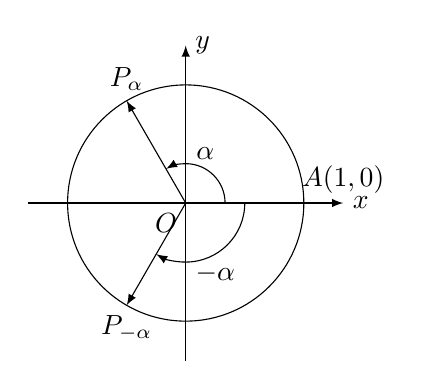
\begin{tikzpicture}[>=latex]
\draw[->] (-2,0)--(2,0)node[right]{$x$};
\draw[->] (0,-2)--(0,2)node[right]{$y$};
\draw (0,0) circle (1.5);
\draw[->](0,0)--(120:1.5)node[above]{$P_{\alpha}$};
\draw[->](0,0)--(-120:1.5)node[below]{$P_{-\alpha}$};
\draw[->] (.5,0) arc (0:120:.5);
\draw[->] (.75,0) arc (0:-120:.75);
\node at (60:.5)[above] {$\alpha$};
\node at (-60:.75)[below] {$-\alpha$};
\node at (2,0)[above]{$A(1,0)$};
\node at (-.25,-.25){$O$};
\end{tikzpicture}
    \caption{}
\end{figure}


设它们的终边与单位圆交于
$P_{\alpha}$和$P_{-\alpha}$ 两点,此两点也必定
关于$Ox$轴对称。

根据三角函数的定义,
\begin{itemize}
    \item $P_{\alpha}$点的坐标是$(\cos\alpha ,\sin\alpha)$;
    \item $P_{-\alpha}$
点的坐标是$(\cos(-\alpha ),\sin(-\alpha ))$。
\end{itemize}

因此,由它们关于$Ox$轴的
对称性便知道它们的横坐标相等,纵坐标是相反数,也就
是说
\[\cos(-\alpha )=\cos\alpha ,\qquad \sin(-\alpha )= -\sin\alpha\]

由此,
\[\begin{split}
    \tan(-\alpha)&=\frac{\sin(-\alpha)}{\cos(-\alpha)}=\frac{-\sin\alpha}{\cos\alpha}=-\tan\alpha\\
    \cot(-\alpha)&=\frac{\cos(-\alpha)}{\sin(-\alpha)}=\frac{\cos\alpha}{-\sin\alpha}=-\cot\alpha\\
\end{split}\]
\end{proof}

\begin{example}
求$\cos\left(-\frac{\pi}{6}\right)$,$\sin \left(-\frac{\pi}{6}\right)$,$\tan\left(-\frac{\pi}{6}\right)$,$\cot\left(-\frac{\pi}{6}\right)$的值。    
\end{example}

\begin{solution}
\[\begin{split}
\cos\left(-\frac{\pi}{6}\right)&=\cos\frac{\pi}{6}=\frac{\sqrt{3}}{2}  \\
\sin\left(-\frac{\pi}{6}\right)&=-\sin\frac{\pi}{6}=-\frac{1}{2} \\
\tan\left(-\frac{\pi}{6}\right)&=-\tan\frac{\pi}{6}=-\frac{\sqrt{3}}{3}   \\
\cot\left(-\frac{\pi}{6}\right)&=-\cot\frac{\pi}{6}=-\sqrt{3}
\end{split}\]
\end{solution}

\begin{example}
    下面函数哪些是偶函数,哪些是奇函数,哪些都
不是?
\begin{multicols}{2}
\begin{enumerate}
    \item $g(x)=1-\cos x$
    \item $F(x)=x-\sin x$
    \item $h(x)=x^2\cos x$
    \item $y(x)=\frac{x+\sin x}{x-\sin x}$
\end{enumerate}
\end{multicols}
\end{example}

\begin{solution}
\begin{enumerate}
    \item $\because\quad g(-x)=1-\cos(-x)=1-\cos x=g(x)$
    
    $\therefore\quad g(x)$是偶函数。
    \item $\because\quad F(-x)=(-x)-\sin(-x)=-x-(-\sin x)=-(x-\sin x)=-F(x)$
    
    $\therefore\quad F(x)$是奇函数。
    \item $\because\quad h(-x)=(-x)^2\cos(-x)=x^2\cos x=h(x)$
    
    $\therefore\quad h(x)$是偶函数。
    \item $\because\quad y(-x)=\frac{(-x)+\sin (-x)}{(-x)-\sin (-x)}=\frac{-(x+\sin x)}{-(x-\sin x)}=\frac{x+\sin x}{x-\sin x}=y(x)$
    
    $\therefore\quad y(x)$是偶函数。
\end{enumerate}
\end{solution}

\begin{ex}
    下面函数哪些是偶函数,哪些是奇函数,哪些都不是?
\begin{multicols}{2}
\begin{enumerate}
    \item $f(x) =|\sin x|$
    \item $H(x)=x^2 +\sin x$
    \item $\phi(x)=\cos x\sin x$
    \item $G(x)=\frac{1-\cos x}{1+\cos x}$
    \item $f(t)=\frac{t^2+\sin t^2}{1+\sin^2 t}$
    \item $y=\tan (x+2)$
    \item $y=-\tan 2x+2$
    \item $y=\tan (3-x)$
\end{enumerate}
\end{multicols}
\end{ex}

\subsection{$2\pi\pm\alpha$与$\alpha$的三角函数间的关系}
根据三角函数的定义可以知道,终边相同的角的同一三
角函数的值相等,即
\begin{equation}
\begin{split}
    \sin(\alpha+2k\pi )=\sin\alpha,&\qquad \cos(\alpha+2k\pi )=\cos\alpha \\
\tan(\alpha+2k\pi ) =\tan\alpha,&\qquad \cot(\alpha+2k\pi )=\cot\alpha
\end{split}
\end{equation}
其中$k\in\mathbb{Z}$。

利用上面的公式可以把求任意角的三角函数值的问题,
转化为求0到$2\pi$间角的三角函数值的问题。

\begin{example}
    求下列三角函数值:
\begin{multicols}{3}
\begin{enumerate}
    \item $\sin(-1480^{\circ}10')$
    \item $\cos\left(\frac{9\pi}{4}\right)$
    \item $\tan\left(-\frac{11\pi}{3}\right)$
\end{enumerate}
\end{multicols}
\end{example}

\begin{solution}
\begin{enumerate}
    \item 
$\sin(-1480^{\circ}10')=-\sin(1480^{\circ}10')=-\sin(4\x 360^{\circ}+40^{\circ}10')=-\sin 40^{\circ}10'=-0.6451$
\item $\cos\left(\frac{9\pi}{4}\right)=\cos\left(2\pi+\frac{\pi}{4}\right)=\cos\frac{\pi}{4}=\frac{\sqrt{2}}{2}$
\item $\tan\left(-\frac{11\pi}{3}\right)=\tan\left(-4\pi+\frac{\pi}{3}\right)=\tan\frac{\pi}{3}=\sqrt{3}$
\end{enumerate}
\end{solution}

在上面公式中,若令$k=1$, 则有
\begin{equation}
    \begin{split}
        \sin(2\pi+\alpha)=\sin\alpha,&\qquad \cos(2\pi+\alpha)=\cos\alpha \\
    \tan(2\pi+\alpha) =\tan\alpha,&\qquad \cot(2\pi+\alpha)=\cot\alpha
    \end{split}
    \end{equation}

现在来看$2\pi-\alpha$的各三角函数值:
\[\begin{split}
    \sin(2\pi-\alpha)&=\sin[2\pi+(-\alpha)]=\sin(-\alpha)=-\sin\alpha\\
    \cos(2\pi-\alpha)&=\cos[2\pi+(-\alpha)]=\cos(-\alpha)=\cos\alpha\\
    \tan(2\pi-\alpha)&=\tan[2\pi+(-\alpha)]=\tan(-\alpha)=-\tan\alpha\\
    \cot(2\pi-\alpha)&=\cot[2\pi+(-\alpha)]=\cot(-\alpha)=-\cot\alpha\\    
\end{split}\]

于是有
\begin{equation}
    \begin{split}
        \sin(2\pi-\alpha)=-\sin\alpha,&\qquad \cos(2\pi-\alpha)=\cos\alpha \\
    \tan(2\pi-\alpha) =-\tan\alpha,&\qquad \cot(2\pi-\alpha)=-\cot\alpha
    \end{split}
    \end{equation}

\begin{example}
    求下列各三角函数值:
\begin{multicols}{3}
\begin{enumerate}
    \item $\sin\frac{11\pi}{6}$
    \item $\cos\frac{13\pi}{8}$
    \item $\cot310^{\circ}18'$
    \item $\sin\left(-\frac{17}{3}\pi\right)$
    \item $\tan(-324^{\circ}18')$
\end{enumerate}
\end{multicols}
\end{example}

\begin{solution}
\begin{enumerate}
    \item $\sin\frac{11\pi}{6}=\sin\left(2\pi-\frac{\pi}{6}\right)=-\sin\frac{\pi}{6}=-\frac{1}{2}$
    \item $\cos\frac{13\pi}{8}=\cos\left(2\pi-\frac{3\pi}{8}\right)=\cos\frac{3\pi}{8}=\cos67^{\circ}30'=0.3827$
    \item $\cot310^{\circ}18'=\cot(360^{\circ}-49^{\circ}42')=-\cot49^{\circ}42'=-0.8481$
    \item $\sin\left(-\frac{17}{3}\pi\right)=\sin\left(-6\pi+\frac{\pi}{3}\right)=\sin\frac{\pi}{3}=\frac{\sqrt{3}}{2}$
    
或者
\[\sin\left(-\frac{17}{3}\pi\right)=-\sin\frac{17\pi}{3}=-\sin\left(6\pi-\frac{\pi}{3}\right)=-\sin\left(-\frac{\pi}{3}\right)=\sin\frac{\pi}{3}=\frac{\sqrt{3}}{2}\]

    \item $\tan(-324^{\circ}18')=-\tan324^{\circ}18'=-\tan(360^{\circ}-35^{\circ}42')=-(-\tan 35^{\circ}42')=\tan 35^{\circ}42'=0.7186$
\end{enumerate}    
\end{solution}

\subsection{$\frac{\pi}{2}\pm\alpha$与$\alpha$的三角函数间的关系}

$\frac{\pi}{2}\pm\alpha$与$\alpha$的三角函数间有下述关系:
\begin{equation}
    \begin{split}
\sin\left(\frac{\pi}{2}+\alpha\right)=\cos\alpha,&\qquad \cos\left(\frac{\pi}{2}+\alpha\right)=-\sin\alpha\\
\tan\left(\frac{\pi}{2}+\alpha\right)=-\cot\alpha,&\qquad \cot\left(\frac{\pi}{2}+\alpha\right)=-\tan\alpha        
    \end{split}
\end{equation}

\begin{proof}
    设$P$和$P'$是单位圆上的点,且$\angle POP'=\frac{\pi}{2}$。
    若$P$点分别在第一、二、三、四象限,那么$P'$点就依次在
    第二、三、四、一象限,如图6.17所示。
\begin{figure}[htp]
    \centering
\begin{tikzpicture}[>=latex]
    \draw[->] (-2,0)--(2,0)node[right]{$x$};
    \draw[->] (0,-2)--(0,2)node[right]{$y$};
    \draw (0,0) circle (1.5);
\draw [thick](0,0)--(30:1.5)node[right]{$P$}--(1.5*1.732/2,0)node[below]{$M$};
\draw [thick](0,0)--(30+90:1.5)node[above]{$P'$}--(0,1.5*1.732/2)node[right]{$M'$};
\node at (-.25,-.25){$O$};
\draw[->] (1,0) arc (0:30:1)node[right]{$\alpha$};
\draw[->] (.5,0) arc (0:30+90:.5);
\node at (60:.7){$\alpha+\tfrac{\pi}{2}$};
\end{tikzpicture}
    \caption{}
\end{figure}

    从$P$点和$P'$点分别向$Ox$轴和$Oy$轴引垂线$PM$, $P'M'$。从直角三角形$OMP$和$OM'P'$全等得
\[|OM|=|OM'|,\qquad |MP|=|M'P'|\]
    
由上面等式和对于任意角$\alpha$的$P,P'$两点所在象限知道:$P$点的横坐标$x_P=OM$,恒与$P'$点的纵坐标$y_{P'}=OM'$相等,即它们的绝对值和符号都相同,也就是$x_P=y_{P'}$,因此$\cos\alpha=\sin\left(\alpha+\frac{\pi}{2}\right)$。

又$P$点的纵坐标$y_P=MP$是$P'$点的横坐标$x_{P'}=M'P'$的相反数,即$y_P=MP=-M'P'=-x_{P'}$,因此,$\sin\alpha=-\cos\left(\alpha+\frac{\pi}{2}\right)$。这样就得到:
\[\begin{split}
    \sin\left(\frac{\pi}{2}+\alpha\right)&=\cos\alpha\\
    \cos\left(\frac{\pi}{2}+\alpha\right)&=-\sin\alpha\\
    \tan\left(\frac{\pi}{2}+\alpha\right)&=\frac{\sin\left(\frac{\pi}{2}+\alpha\right)}{\cos\left(\frac{\pi}{2}+\alpha\right)}=\frac{\cos\alpha}{-\sin\alpha}=-\cot\alpha\\
    \cot\left(\frac{\pi}{2}+\alpha\right)&=\frac{\cos\left(\frac{\pi}{2}+\alpha\right)}{\sin \left(\frac{\pi}{2}+\alpha\right)}=\frac{-\sin\alpha}{\cos\alpha}=-\tan\alpha
\end{split}\]
\end{proof}

由公式(6.7)我们可以得到,对于任意角$\alpha$,
\[\begin{split}
\sin\left(\frac{\pi}{2}-\alpha\right)&=\sin\left[\frac{\pi}{2}+(-\alpha)\right]=  \cos(-\alpha)=\cos\alpha \\
\cos\left(\frac{\pi}{2}-\alpha\right)&=\cos\left[\frac{\pi}{2}+(-\alpha)\right]=  -\sin(-\alpha)=\sin\alpha \\
\tan\left(\frac{\pi}{2}-\alpha\right)&=\tan\left[\frac{\pi}{2}+(-\alpha)\right]= -\cot(-\alpha)=\cot\alpha  \\
\cot\left(\frac{\pi}{2}-\alpha\right)&=\cot\left[\frac{\pi}{2}+(-\alpha)\right]=  -\tan(-\alpha)=\tan\alpha 
\end{split}\]
于是有
\begin{equation}
\begin{split}
    \sin\left(\frac{\pi}{2}-\alpha\right)=\cos\alpha, &\qquad \cos\left(\frac{\pi}{2}-\alpha\right)=\sin\alpha \\
    \tan\left(\frac{\pi}{2}-\alpha\right)=\cot\alpha, &\qquad \cot\left(\frac{\pi}{2}-\alpha\right)=\tan\alpha 
\end{split}    
\end{equation}

\subsection{$\pi\pm\alpha$、$\frac{3\pi}{2}\pm \alpha$与$\alpha$的三角函数间的关系}
由于
\[\begin{split}
\sin(\pi+\alpha)&=\sin \left[\frac{\pi}{2}+\left(\frac{\pi}{2}+\alpha\right)\right]=\cos\left(\frac{\pi}{2}+\alpha\right)=-\sin\alpha\\
\cos(\pi+\alpha)&=\cos \left[\frac{\pi}{2}+\left(\frac{\pi}{2}+\alpha\right)\right]=-\sin\left(\frac{\pi}{2}+\alpha\right)=-\cos\alpha\\
\tan(\pi+\alpha)&=\tan \left[\frac{\pi}{2}+\left(\frac{\pi}{2}+\alpha\right)\right]=-\cot\left(\frac{\pi}{2}+\alpha\right)=-(-\tan\alpha)=\tan\alpha\\
\cot(\pi+\alpha)&=\cot \left[\frac{\pi}{2}+\left(\frac{\pi}{2}+\alpha\right)\right]=-\tan\left(\frac{\pi}{2}+\alpha\right)=-(-\cot\alpha)=\cot\alpha\\
\end{split}\]
因此有:
\begin{equation}
    \begin{split}
        \sin\left(\pi+\alpha\right)=-\sin\alpha, &\qquad \cos\left(\pi+\alpha\right)=-\cos\alpha \\
        \tan\left(\pi+\alpha\right)=\tan\alpha, &\qquad \cot\left(\pi+\alpha\right)=\cot\alpha 
    \end{split}    
    \end{equation}

由于
\[\begin{split}
\sin(\pi-\alpha)&=\sin[\pi+(-\alpha)]= -\sin(-\alpha)=\sin\alpha\\
\cos(\pi-\alpha)&=\cos[\pi+(-\alpha)]= -\cos(-\alpha)=-\cos\alpha\\
\tan(\pi-\alpha)&=\tan[\pi+(-\alpha)]= \tan(-\alpha)=-\tan\alpha\\
\cot(\pi-\alpha)&=\cot[\pi+(-\alpha)]= \cot(-\alpha)=-\cot\alpha\\
\end{split}\]
因此有:
\begin{equation}
    \begin{split}
        \sin\left(\pi-\alpha\right)=\sin\alpha, &\qquad \cos\left(\pi-\alpha\right)=-\cos\alpha \\
        \tan\left(\pi-\alpha\right)=-\tan\alpha, &\qquad \cot\left(\pi-\alpha\right)=-\cot\alpha 
    \end{split}    
    \end{equation}

由于
\[\begin{split}
\sin\left(\frac{3\pi}{2}+\alpha\right)&=\sin \left[\pi+\left(\frac{\pi}{2}+\alpha\right)\right]=-\sin\left(\frac{\pi}{2}+\alpha\right)=-\cos\alpha\\
\cos\left(\frac{3\pi}{2}+\alpha\right)&=\cos \left[\pi+\left(\frac{\pi}{2}+\alpha\right)\right]=-\cos\left(\frac{\pi}{2}+\alpha\right)=-(-\sin\alpha)=\sin\alpha\\
\tan\left(\frac{3\pi}{2}+\alpha\right)&=\tan \left[\pi+\left(\frac{\pi}{2}+\alpha\right)\right]=\tan\left(\frac{\pi}{2}+\alpha\right)=-\cot\alpha\\
\cot\left(\frac{3\pi}{2}+\alpha\right)&=\cot \left[\pi+\left(\frac{\pi}{2}+\alpha\right)\right]=\cot\left(\frac{\pi}{2}+\alpha\right)=-\tan\alpha
\end{split}\]
因此有:
\begin{equation}
    \begin{split}
        \sin\left(\frac{3\pi}{2}+\alpha\right)=-\cos\alpha, &\qquad \cos\left(\frac{3\pi}{2}+\alpha\right)=\sin\alpha \\
        \tan\left(\frac{3\pi}{2}+\alpha\right)=-\cot\alpha, &\qquad \cot\left(\frac{3\pi}{2}+\alpha\right)=-\tan\alpha 
    \end{split}    
    \end{equation}

由于
\[\begin{split}
\sin\left(\frac{3\pi}{2}-\alpha\right)&=\sin\left[\frac{3\pi}{2}+(-\alpha)\right]=-\cos(-\alpha)=-\cos\alpha\\
\cos\left(\frac{3\pi}{2}-\alpha\right)&=\cos \left[\frac{3\pi}{2}+(-\alpha)\right]=\sin(-\alpha)=-\sin\alpha\\
\tan\left(\frac{3\pi}{2}-\alpha\right)&=\tan \left[\frac{3\pi}{2}+(-\alpha)\right]=-\cot(-\alpha)=\cot\alpha\\
\cot\left(\frac{3\pi}{2}-\alpha\right)&=\cot \left[\frac{3\pi}{2}+(-\alpha)\right]=-\tan(-\alpha)=\tan\alpha
\end{split}\]

因此有:
\begin{equation}
    \begin{split}
        \sin\left(\frac{3\pi}{2}-\alpha\right)=-\cos\alpha, &\qquad \cos\left(\frac{3\pi}{2}-\alpha\right)=-\sin\alpha \\
        \tan\left(\frac{3\pi}{2}-\alpha\right)=\cot\alpha, &\qquad \cot\left(\frac{3\pi}{2}-\alpha\right)=\tan\alpha 
    \end{split}    
    \end{equation}

\begin{example}
求$\sin(-1650^{\circ})$,$\cos\left(-\frac{19\pi}{6}\right)$的值。
\end{example}

\begin{solution}
\[\begin{split}
    \sin(-1650^{\circ})&=-\sin(1650^{\circ})=-\sin(4\x360^{\circ}+210^{\circ})\\
    &=-\sin 210^{\circ}=-\sin(180^{\circ}+30^{\circ})\\
    &=\sin30^{\circ}=\frac{1}{2}
\end{split}\]
\[\begin{split}
    \cos\left(-\frac{19\pi}{6}\right)&=\cos\frac{19\pi}{6}=\cos\left(2\pi+\frac{7\pi}{6}\right)\\
    &=\cos\frac{7\pi}{6}=\cos\left(\pi+\frac{\pi}{6}\right)\\
    &=-\cos\frac{\pi}{6}=-\frac{\sqrt{3}}{2}
\end{split}\]
\end{solution}

\subsection{三角函数的诱导公式}

把上面的自变数是$-\alpha$、$\frac{\pi}{2}\pm\alpha$、$\pi\pm\alpha$、$\frac{3\pi}{2}\pm\alpha$、$2\pi\pm\alpha$
的三角函数表示为自变数就是$\alpha$的三角函数的公式,
叫做三角函数的诱导公式。为便于查阅和比较,我们把三角
函数的诱导公式全部都列于下表中。
\begin{center}
\begin{tabular}{ccccc}
    \hline
& $\cos$ & $\sin$ & $\tan $ &  $\cot$\\
\hline
$-\alpha$& $\cos\alpha$ & $-\sin\alpha$ & $-\tan\alpha $ &  $-\cot\alpha$\\
\vspace{1ex}$\frac{\pi}{2}+\alpha$& $-\sin\alpha$ & $\cos\alpha$ & $-\cot\alpha $ &  $-\tan\alpha$\\
\vspace{1ex}$\frac{\pi}{2}-\alpha$& $\sin\alpha$ & $\cos\alpha$ & $\cot\alpha $ &  $\tan \alpha$\\
$\pi+\alpha$& $-\cos\alpha$ & $-\sin\alpha$ & $\tan\alpha $ &  $\cot\alpha$\\
$\pi-\alpha$& $-\cos\alpha$ & $\sin\alpha$ & $-\tan\alpha $ &  $-\cot\alpha$\\
\vspace{1ex}$\frac{3\pi}{2}+\alpha$& $\sin\alpha$ & $-\cos\alpha$ & $-\cot\alpha $ &  $-\tan\alpha$\\
\vspace{1ex}$\frac{3\pi}{2}-\alpha$& $-\sin\alpha$ & $-\cos\alpha$ & $\cot\alpha $ &  $\tan\alpha$\\
$2\pi+\alpha$& $\cos\alpha$ & $\sin\alpha$ & $\tan\alpha $ &  $\cot\alpha$\\
$2\pi-\alpha$& $\cos\alpha$ & $-\sin\alpha$ & $-\tan\alpha $ &  $-\cot\alpha$\\
\hline
\end{tabular}
\end{center}

比如要计算$\tan\left(\frac{\pi}{2}+\alpha\right)$
的值,在表中找到标记$\frac{\pi}{2}+\alpha$
的第二行与标记$\tan$的第三列,它们相交之处,标记着
$-\cot\alpha$, 于是,相应的诱导公式可以写成
$\tan \left(\frac{\pi}{2}+\alpha\right) =
-\cot\alpha$。

表中最后一列,给出对于锐角$\alpha$ (带斜条的全等直角三
角形的顶点在圆心的锐角)的三角函数诱导公式的几何解
释。

我们称正弦与余弦,正切与余切互为余函数。

从表中,可知$-\alpha$、$\frac{\pi}{2}\pm\alpha$、$\pi \pm\alpha$、
$\frac{3\pi}{2}\pm \alpha$ 和$2\pi \pm\alpha$ 都可以化成$k\frac{\pi}{2}
\pm\alpha$ $(k=0,1,2,3,4)$ 的形式,并且
这些角的三角函数和角$\alpha$ 的三角函数之间的关系,可以总结
出下面的法则。

\begin{enumerate}
    \item 符号
    
要确定结果的符号,只要假定$\alpha$为锐角(实际上,在所
有公式中的$\alpha$ 都是任意角),看角$k\cdot \frac{\pi}{2}\pm \alpha$在哪一象限,然后用原来函数在这个象限内应取的符号,作为结果的符号。

\item 函数名称
\begin{enumerate}
    \item 若$k$为偶数(包括$k=0$在内)则等式两边函数名称相同。
    \item 若$k$为奇数,则等式两边函数名称不同,可由原来
函数名称中的“正”变“余”,或“余”变“正”(就是正
弦变余弦,正切变余切;或余弦变正弦,余切变正切等等)
而得到。
\end{enumerate}
\end{enumerate}

为了便于记忆,上述法则还可以概括成下面的口诀:
\begin{center}
\verb|正负看象限,奇变偶不变。 |
\end{center}

利用上面的法则,便可以迅速地写出三角函数的诱导公
式,下面举例来说明。

\begin{example}
    写出$\cos\left(\frac{3\pi}{2}+\alpha\right)$的诱导公
    式。
\end{example}

\begin{solution}
\begin{enumerate}
    \item 假定$\alpha$ 是锐角,则
$\frac{3\pi}{2}+\alpha$ 是第四象限的
角,而第四象限的角的余弦是正的,所以结果应取正号。
\item 因为$\frac{3\pi}{2}=3\cdot \frac{\pi}{2}$,3是奇数,所以,结果中函数名称应由余弦变为正弦,因此,有
\[\cos\left(\frac{3\pi}{2}+\alpha\right)=\cos\left(3\cdot \frac{\pi}{2}+\alpha\right)=\sin\alpha\]
\end{enumerate}
\end{solution}

\begin{example}
    写出$\tan(\pi-\alpha)$的诱导公式。
\end{example}

\begin{solution}
\begin{enumerate}
    \item 假定$\alpha$是锐角,则
$\pi -\alpha$ 是第二象限的角,
而第二象限的角的正切是负的,所以结果应取负号。
\item 因为$\pi =2\cdot\frac{\pi}{2}$,2是偶数,所以,结果中
函数名称与原来的相同,仍为正切,因此,有
\[\tan(\pi -\alpha )=-\tan\alpha \]
\end{enumerate}
\end{solution}

利用三角函数的诱导公式,我们可以把求任意角的三角
函数值的问题化为求锐角三角函数值的问题。下面分三种情
形举例说明。

第一种情形:0到$2\pi$ (或$0^{\circ}$到$360^{\circ}$)之间的角的三角
函数。先选用适当的诱导公式化为锐角函数,然后求值。

\begin{example}
\[\sin 150^{\circ}=\sin(180^{\circ}-30^{\circ})=\sin30^{\circ}=\frac{1}{2}\]
或
  \[\sin 150^{\circ}=\sin(90^{\circ}+60^{\circ})=\cos60^{\circ}=\frac{1}{2}\]  
\end{example}

\begin{example}
\[\cos\frac{2\pi}{3}=\cos\left(\pi-\frac{\pi}{3}\right)=-\cos\frac{\pi}{3}=-\frac{1}{2}\]
或
\[\cos\frac{2\pi}{3}=\cos\left(\frac{\pi}{2}+\frac{\pi}{6}\right)=-\sin\frac{\pi}{6}=-\frac{1}{2}\]
\end{example}

\begin{example}
    $\tan\frac{4\pi}{3}=\tan\left(\pi+\frac{\pi}{3}\right)=\tan\frac{\pi}{3}=\sqrt{3}$
\end{example}

\begin{example}
$\cot313^{\circ}25'=\cot(360^{\circ}-46^{\circ}35')=-\cot46^{\circ}35'=-0.9463$
\end{example}

第二种情形:大于$2\pi$ (或大于$360^{\circ}$) 的角的三角函数,
可利用公式(6.4), 化为上述第一种情形,然后求值。

\begin{example}
    $\sin 510^{\circ}=\sin(360^{\circ}+150^{\circ})=\sin150^{\circ}=\sin30^{\circ}=\frac{1}{2}$
\end{example}


\begin{example}
    $\cos\frac{8\pi}{3}=\cos\left(2\pi+\frac{2\pi}{3}\right)=\cos\frac{2\pi}{3}=\cos\left(\pi-\frac{\pi}{3}\right)=-\cos\frac{\pi}{3}=-\frac{1}{2}$
\end{example}

\begin{example}
\[\begin{split}
    \tan500^{\circ}=\tan(360^{\circ}+140^{\circ})&=\tan 140^{\circ}\\
    &=\tan(180^{\circ}-40^{\circ})\\ &=-\tan40^{\circ}=-0.8391
\end{split}\]
\end{example}

第三种情形:负角的三角函数,可先化为正角的三角函
数,然后再分别按上述两种情形求值。

\begin{example}
\[\begin{split}
    \sin( -680^{\circ}) &= -\sin680^{\circ} =-\sin(360^{\circ}+320^{\circ})\\
   &=-\sin320^{\circ}
   =-\sin(360^{\circ}-40^{\circ})\\
  & =-(-\sin40^{\circ})   =\sin40^{\circ}=0.6428
\end{split}\]
或$$\sin( -680^{\circ})=\sin( -680^{\circ}+2\x 360^{\circ})=\sin 40^{\circ}=0.6428$$
\end{example}

\begin{example}
    \[\begin{split}
        \cos\left(-\frac{22\pi}{5}\right)=\cos\frac{22\pi}{5}&=\cos\left(4\pi+\frac{2\pi}{5}\right)\\ &=\cos\frac{2\pi}{5}=\cos72^{\circ}=0.3090
    \end{split}\]
\end{example}    


\begin{example}
    化$\tan (\alpha-270^{\circ})$为角$\alpha$的三角函数。
\end{example}

\begin{solution}
$$\tan (\alpha-270^{\circ})=\tan [-(270^{\circ}-\alpha)]
=-\tan (270^{\circ}-\alpha)
=-\cot \alpha$$
或
$$\tan (\alpha-270^{\circ})=\tan[ (\alpha-270^{\circ})+360^{\circ}]
=\tan (90^{\circ}+\alpha)=-\cot \alpha$$
\end{solution}

\section*{习题6.1}
\addcontentsline{toc}{subsection}{习题6.1}
\begin{enumerate}
    \item 用余角的三角函数来替换下面的三角函数。
\begin{multicols}{2}
\begin{enumerate}
    \item $\sin75^{\circ}30'$
    \item $\sin(30^{\circ}-\alpha)$
    \item $\cos(2\alpha+14^{\circ})$
    \item $\cos\left(\frac{\alpha}{2}+55^{\circ}\right)$
    \item $\tan\left(66^{\circ}-\frac{\alpha}{3}\right)$
    \item $\cot(45^{\circ}+\alpha)$
\end{enumerate}
\end{multicols}
    \item 查表求下列三角函数值:
\begin{multicols}{2}
    \begin{enumerate}
        \item $\sin105^{\circ}45'$
        \item $\cos165^{\circ}24'$
        \item $\tan200^{\circ}$
        \item $\cot290^{\circ}$
    \end{enumerate}
    \end{multicols}
    \item 查表求下列三角函数值:
\begin{multicols}{2}
\begin{enumerate}
    \item $\sin\frac{5\pi}{8}$
    \item $\cos\frac{9\pi}{8}$
    \item $\tan 1.4\pi$
    \item $\cot 1.8\pi$
    \item $-\tan 0.3\pi$
\end{enumerate}
\end{multicols}

\item 查表求下列三角函数值:
\begin{multicols}{2}
\begin{enumerate}
    \item $\sin(-1640^{\circ})$
    \item $\cos(-900^{\circ})$
    \item $\tan(-700^{\circ})$
    \item $\cot\left(-13\frac{3}{4}\pi\right)$
\end{enumerate}
\end{multicols}

\item 查表求下列三角函数值:
\begin{multicols}{2}
\begin{enumerate}
    \item $\sin2$
    \item $\cos1$
    \item $\tan(-3)$
    \item $\cot(\sin2)$
\end{enumerate}
\end{multicols}
\item 查表求下列三角函数值:
\begin{multicols}{2}
\begin{enumerate}
    \item $\sin 1160^{\circ}$
    \item $\tan (-1596^{\circ})$
    \item $\cot 864^{\circ}$
    \item $\cos(-320^{\circ})$
    \item $\tan 1190^{\circ}$
    \item $\cos(-847^{\circ}32')$
    \item $-\sin 570^{\circ}$
    \item $-\cot 390^{\circ}$
\end{enumerate}
\end{multicols}

\item 已知$\sin(180^{\circ}+\alpha)=-\frac{1}{2}$,计算:
\begin{multicols}{2}
\begin{enumerate}
    \item $\sin(270^{\circ}+\alpha)$
    \item $\cos(90^{\circ}+\alpha)$
    \item $\tan(\alpha-270^{\circ})$
    \item $\tan(\alpha-180^{\circ})$
\end{enumerate}
\end{multicols}
\item 计算下列各式的值:
\begin{enumerate}
    \item $2\sin^2\frac{17\pi}{4}+\tan^2\frac{33\pi}{4}\cot\frac{3\pi}{4}$
    \item $\tan10^{\circ}\cdot \tan20^{\circ}\cdot \tan30^{\circ}\cdot \tan40^{\circ}\cdot \tan50^{\circ}\cdot \tan60^{\circ}\cdot \tan70^{\circ}\cdot \tan80^{\circ}$
    \item $\sin110^{\circ}+\sin130^{\circ}+\sin150^{\circ}+\sin170^{\circ}+\sin190^{\circ}+\sin210^{\circ}+\sin230^{\circ}+\sin250^{\circ}+\sin270^{\circ}$
\end{enumerate}


\item 确定下列各式的符号:
\begin{multicols}{2}
\begin{enumerate}
    \item $\sin 100^{\circ}+\cos100^{\circ}$
    \item $\frac{1}{\cos230^{\circ}}-\frac{1}{\cos220^{\circ}}$
\end{enumerate}
\end{multicols}

\item 查表求角,若
\begin{enumerate}
    \item $\sin\alpha=-0.515,\qquad 180^{\circ}<\alpha<270^{\circ}$
    \item $\sin\alpha=0.669,\qquad 90^{\circ}<\alpha<180^{\circ}$
    \item  $\tan\alpha=-1.376,\qquad 90^{\circ}<\alpha<180^{\circ}$
    \item $\cos\alpha=0.407,\qquad 270^{\circ}<\alpha<360^{\circ}$
    \item $\tan\alpha=0.577,\qquad 180^{\circ}<\alpha<270^{\circ}$
    \item $\cot\alpha=-2.747,\qquad 90^{\circ}<\alpha<180^{\circ}$
\end{enumerate}
\end{enumerate}

\subsection{正切函数线与余切函数线}
\begin{blk}{定义}
    过单位圆与坐标系的横轴$Ox$的交点$A(1,0)$的切
线叫做正切函数线,简称正切线;而过单位圆与坐标系纵轴
$Oy$的交点$B(0,1)$的切线叫做余切函数线,简称余切线(图
6.18)。
\end{blk}

\begin{figure}[htp]
    \centering
\begin{tikzpicture}[>=latex]
\draw[->](-2,0)--(2.5,0)node[right]{$x$};
\draw[->](0,-2)--(0,2.5)node[right]{$y$};
\draw (0,0) circle(1.5);
\draw[thick] (-2,1.5)--(2,1.5)node[right]{余切线};
\draw[thick] (1.5,-2)node[below]{正切线}--(1.5,2);
\node at (-.25,-.25){$O$};
\node at (2,0)[below]{$A(1,0)$};
\node at (.5,1.5)[above]{$B(0,1)$};

\end{tikzpicture}
    \caption{}
\end{figure}


正切线与$Oy$轴平行,在正
切线上,规定它的正方向与$Oy$
轴的正方向一致,它上面的单
位长等于单位圆的半径。

令$P$是角$\alpha$的终边与单位
圆的交点,延长旋转半径$OP$或反向延长旋转半径$OP$与正
切线交于$L$点(当$P$点位于
$Oy$轴上时,过$O$、$P$两点的直线就不与正切线相交),如
图6.19所示。


\begin{blk}{定理}
    角$\alpha$的正切等于它的终边所在直线与正切线的交
点的纵坐标。
\end{blk}

\begin{proof}
    如果角$\alpha$的终边$OP$在$Oy$轴的右侧,射线$OP$
    与正切线交于$L$点。设$P$点坐标为$(x,y)$, $L$点坐标为$(1,y_1)$,这时
\[\tan\alpha=\frac{y}{x}=\frac{AL}{1}=y_1\]
这里$AL$是有向线段$\Vec{AL}$的数量(图6.19(a))。

\begin{figure}[htp]
    \centering
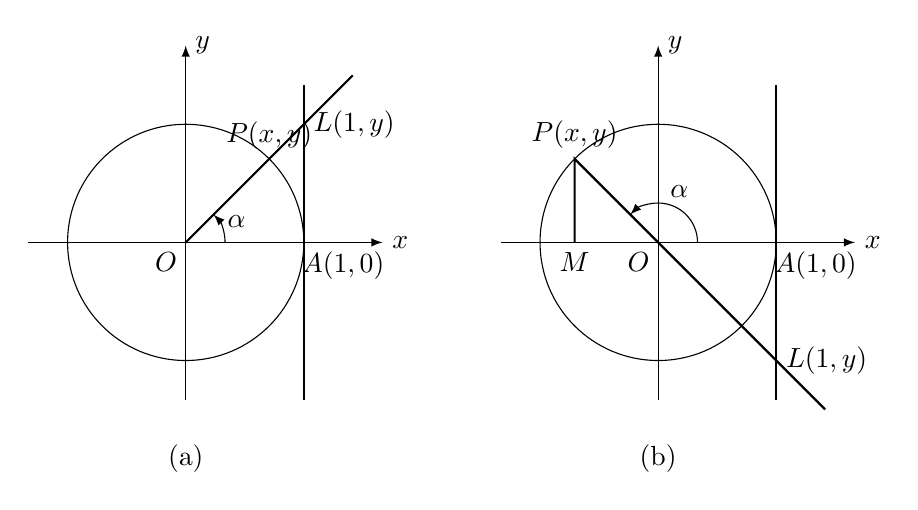
\begin{tikzpicture}[>=latex]
\begin{scope}
\draw[->](-2,0)--(2.5,0)node[right]{$x$};
\draw[->](0,-2)--(0,2.5)node[right]{$y$};
\draw (0,0) circle(1.5);
\draw[thick] (1.5,-2)--(1.5,2);
\node at (-.25,-.25){$O$};
\node at (2,0)[below]{$A(1,0)$};
\draw[thick] (0,0)--(45:3);
\node at (1.5,1.5)[right]{$L(1,y)$};
\node at (45:1.5)[above]{$P(x,y)$};
\draw[->] (.5,0) arc (0:45:.5);
\node at (45/2:.7) {$\alpha$};
\node at (0,-2.75){(a)};
\end{scope}
\begin{scope}[xshift=6cm]
\draw[->](-2,0)--(2.5,0)node[right]{$x$};
\draw[->](0,-2)--(0,2.5)node[right]{$y$};
\draw (0,0) circle(1.5);
\draw[thick] (1.5,-2)--(1.5,2);
\node at (-.25,-.25){$O$};
\node at (2,0)[below]{$A(1,0)$};
\draw[thick] (-1.5/1.414,0)node[below]{$M$}--(90+45:1.5)node[above]{$P(x,y)$}--(0,0)--(-45:3);
\node at (1.5,-1.5)[right]{$L(1,y)$};
\draw[->] (.5,0) arc (0:45+90:.5);
\node at (135/2:.7){$\alpha$};
\node at (0,-2.75){(b)};
\end{scope}
\end{tikzpicture}
    \caption{}
\end{figure}

如果角$\alpha$ 的终边$OP$在$Oy$轴的左侧,反向延长$OP$与
正切线交于$L$点.设$P$点、$L$点的坐标分别是$(x,y)$、$(x_1,y_1)$,
这时$P$点和$L$点的同名称坐标的符号相反,但由于
$\triangle  OPM    \sim \triangle OLA$, 所以它们的坐标的比相同(图6.19(b)),即
\[\tan\alpha =\frac{y}{x}=\frac{MP}{OM}=\frac{AL}{OA}=\frac{y_1}{1}=y_1\]

如果$P$点在$Oy$轴上则$L$点不存在,$\tan\alpha$ 不存在。

余切线与$Ox$轴平行,在余切线上,规定它的正方向与
$Ox$轴的正方向一致,它上面的单位长等于单位圆的半径。
\end{proof}

我们可以用同样的方法证明下面的定理。































\begin{example}
    
\end{example}

\begin{example}
    
\end{example}

\begin{example}
    
\end{example}

\begin{solution}
    
\end{solution}

\begin{solution}
    
\end{solution}

\begin{solution}
    
\end{solution}

\begin{solution}
    
\end{solution}

\begin{example}
    
\end{example}

\begin{example}
    
\end{example}

\begin{example}
    
\end{example}

\begin{example}
    
\end{example}

\begin{example}
    
\end{example}

\begin{example}
    
\end{example}

\begin{example}
    
\end{example}

\begin{example}
    
\end{example}

\begin{example}
    
\end{example}

\begin{example}
    
\end{example}

\begin{example}
    
\end{example}

\begin{example}
    
\end{example}

\begin{example}
    
\end{example}

\begin{example}
    
\end{example}

\begin{example}
    
\end{example}

\begin{example}
    
\end{example}

\begin{example}
    
\end{example}

\begin{example}
    
\end{example}

\begin{example}
    
\end{example}

\begin{example}
    
\end{example}

\begin{example}
    
\end{example}
\begin{example}
    
\end{example}